% This is the chapter for applying MENP framework to spectrum sensing.
\chapter{Application of MENP Framework in Spectrum Sensing and Simulation Results}
Upon examination of theoretical aspect of the MENP framework and the M-ROC, this thesis will now apply the new hypotheses testing framework to spectrum sensing for multiple primary users. We consider energy as well as cyclostationary based detectors to detect multiple primary signals. Performance analysis results, which illustrate the performance of both detectors, will be presented. 
%----------------------------------------------------------------------------------------------

\typeout{}
% Energy based spectrum sensing
\section{Energy based Spectrum Detector for Multiple Primary Users}
\subsection{System Model}
We consider a cognitive radio system where the licensed frequency spectrum could be occupied by one of two distinct signals $\{s_A, s_B\}$ or it could be vacant. Let $H_0$ denote the hypothesis under which the channel is free, ${H}_1$ denote the hypothesis under which the channel is occupied by $s_A$ and ${H}_2$ denote the hypothesis under which the channel is occupied by $s_B$. We are interested to test $H_0$ against $\bar{{H}_0}$, where $\bar{H}_0$ denotes the hypothesis under which the channel is not free, using MENP framework.

A block diagram of the system is illustrated in Figure \ref{pic: block diagram}.

\begin{figure}[!hbp]
\centering
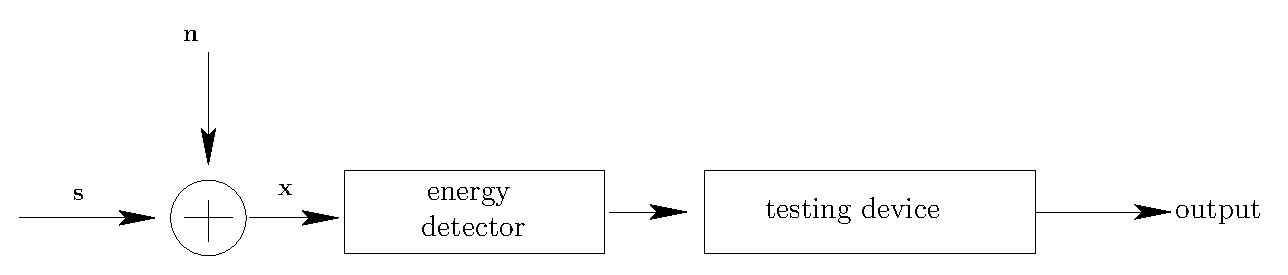
\includegraphics[width = \textwidth]{4/fig4.eps}
\caption{Block Diagram for Spectrum Sensing}
\label{pic: block diagram}
\end{figure}

The detector consists of a measuring device followed by a testing device. 
The measuring device observes the noisy version of the received signals and forms the energy of their sampled version.
With this energy, the testing device employs the MENP framework to decide about the state of the channel.
The input to the measuring device is 
\begin{equation}
  \mathbf{x} = \begin{cases}
	\mathbf{n}\;\;\;\;\;\;&\text{when $H_0$ is true}\\
	\mathbf{n}+\mathbf{s}_A\;\;\;\;\;\;&\text{when $H_1$ is true}\\
	\mathbf{n}+\mathbf{s}_B\;\;\;\;\;\;&\text{when $H_2$ is true}\\
  \end{cases}
  \label{equ:1222n0}
\end{equation}
where 
\begin{equation}
  \begin{cases}
	&\mathbf{x} = (x_0, x_1, \cdots, x_{N-1})\\
	&\mathbf{s}_A = (s_{A0}, s_{A1}, \cdots, s_{A(N-1)})\\
	&\mathbf{s}_B = (s_{B0}, s_{B1}, \cdots, s_{B(N-1)})\\
	&\mathbf{n} = (n_{0}, n_{1}, \cdots, n_{N-1})\,.
  \end{cases}
  \label{1222n1}
\end{equation}

We assume  $s_{A_i}$ $s_{B_i}$ and $n_i$ are zero-mean independent and identically distributed (iid) circularly symmetric complex Gaussian (CSCG) random variables with variances $2\sigma_{s_A}^2$, $2\sigma_{s_B}^2$ and $2\sigma_{n}^2$, i.e., $s_{A_i} \sim \mathcal{CN}(0, 2\sigma_{s_A}^2)$, $s_{B_i} \sim \mathcal{CN}(0, 2\sigma_{s_B}^2)$ and $n_i \sim \mathcal{CN}(0, 2\sigma_{n}^2)$.
Each noisy sample $x_i = s_i + n_i$ is governed by a probability law under each hypothesis. In our model
since the noise and signal are independent, $s_i+ n_i \sim \mathcal{CN}(0, 2(\sigma_{s}^2 + \sigma_n^2))$.  Define $\sigma_0^2 = \sigma_n^2$, $\sigma_1^2 = \sigma_{s_A}^2 + \sigma_n^2$ and $\sigma_2^2 = \sigma_{s_B}^2 + \sigma_n^2$, we can see
\begin{equation}
  \label{1129a1}
  \begin{split}
  n_i &\sim \mathcal{CN}(0, 2\sigma_0^2)\\
  n_i + s_{A_i} &\sim \mathcal{CN}(0, 2\sigma_1^2)\\
   n_i + s_{B_i}&\sim \mathcal{CN}(0, 2\sigma_2^2) \,,
  \end{split}
\end{equation}
thus the distribution of $x_i$ under each hypothesis is given by
\begin{equation}
   \begin{split}
  H_0:\;\;\;\;\begin{pmatrix} x_{i_R} \\ x_{i_I} \end{pmatrix} \sim \mathcal{N}\Big( \begin{bmatrix} 0 \\ 0 \end{bmatrix}, \begin{bmatrix} \sigma_0^2 & 0\\ 0 & \sigma_0^2 \end{bmatrix} \Big)\\
  H_1:\;\;\;\;\begin{pmatrix} x_{i_R} \\ x_{i_I} \end{pmatrix} \sim \mathcal{N}\Big( \begin{bmatrix} 0 \\ 0 \end{bmatrix}, \begin{bmatrix} \sigma_1^2 & 0\\ 0 & \sigma_1^2 \end{bmatrix} \Big)\\
  H_2:\;\;\;\;\begin{pmatrix} x_{i_R} \\ x_{i_I} \end{pmatrix} \sim \mathcal{N}\Big( \begin{bmatrix} 0 \\ 0 \end{bmatrix}, \begin{bmatrix} \sigma_2^2 & 0\\ 0 & \sigma_2^2 \end{bmatrix} \Big)
\end{split}
  \label{equ:xdistribution}
\end{equation}
where $x_{i_R}$ and $x_{i_I}$ are real and imaginary components of $x_i$.
In our case, the measuring device is an energy detector, with output 
\begin{equation} 
  Y = \sum_{i=0}^{N-1}|x_i|^2 = \sum_{i=0}^{N-1}(x_{i_R}^2+x_{i_I}^2)\,.
  \label{equ: testing device}
\end{equation}
By observing $y$, a realization of $Y$, the testing device determines the status of the channel. 
Since $x_{i_R}, x_{i_I}$ are uncorrelated Gaussian random variable with zero mean and variance $\sigma_i^2$, $\frac{y}{\sigma_i^2} = \sum_{n=0}^{N-1}((\frac{x_{i_R}}{\sigma_i})^2 + (\frac{x_{I_i}}{\sigma_i})^2)$ is governed by a Chi-Square distribution with $2N$ degree of freedom under hypothesis $H_i$.
Hence the distribution of $Y$ can be expressed as:
\begin{equation} 
  \label{equ: abstract}
  \begin{split}
	H_0:\;\;\;\;&\frac{Y}{\sigma_0^2}\sim \mathcal{X}(2N)\\
	H_1:\;\;\;\;&\frac{Y}{\sigma_1^2}\sim \mathcal{X}(2N)\\
	H_2:\;\;\;\;&\frac{Y}{\sigma_2^2}\sim \mathcal{X}(2N)\,,
  \end{split}
\end{equation}
where $\mathcal{X}(2N)$ is the Chi-square distribution with $2N$ degrees of freedom. 

Let $P_d$ denote the probability of detection, i.e. the probability that the channel is correctly declared vacant ($H_0$ is correctly declared true) and $P_{f_1}$ $P_{f_2}$ denote the probability of false alarm with respect to $s_A$  and $s_B$, i.e. the probability that the channel is declared vacant when signal $s_A$ ($s_B$) is present. Let $c_i$ ($i = 1, 2$) denotes the specific positive constraints on the probability of false alarm. The performance of the system can be depicted by $P_d$ and $c_i$ ($i = 1, 2$), and we use the MENP framework to solve following optimization problem:
\begin{equation}
  \begin{split}
	\max\;\;\;\;&P_d\\
	\text{s.t.}\;\;\;\;&P_{f_1}\leq c_1\\
	&P_{f_2} \leq c_2\,.
  \end{split}
  \label{1129a3}
\end{equation}
Our goal is to plot M-ROC surface and to find the decision rule for a given $c_1, c_2$ value.

\subsection{Numerical Results}
Assume $\sigma_n^2=0.1$ $\sigma_{s_A}^2=0.05$ $\sigma_{s_B}^2=0.1$ and $N=20$. We can see $\sigma_0^2=0.1$ $\sigma_1^2=0.15$ and $\sigma_2^2=0.25$, 
thus $\sigma_0^2 < \sigma_1^2, \sigma_2^2$. Hence the problem given in \eqref{1129a3} for hypotheses \eqref{equ: abstract} has the same form as that of Chi-Square Example given in chapter 3. 
If $y$ is an observation of $Y$, 
from the conclusion in chapter 3 the optimal  decision rule for a given $c_1, c_2$ is 
\begin{equation}
  y \substack{H_0 \\ < \\ > \\ \bar{H}_0} V_\tau
  \label{equ:1129a4}
\end{equation}
where 
\begin{equation}
  V_\tau = \min\{F_1^{-1}(c_1),  F_2^{-1}(c_2)\}
  \label{equ:2015may1a2}
\end{equation}
and function $F_1,  F_2$ are the CDFs of $Y$ under hypothesis $H_1, H_2$ respectively. The expression of $P_d$ is 
\begin{equation}
  P_d = F_0(V_\tau)\,.
  \label{equ:1129a5}
\end{equation}

Similar to energy detection in binary hypothesis testing, energy detection for multiple hypothesis testing differentiates between $H_0$ and $\bar{H}_0$ by comparing the test statistic (in form of energy) with a threshold $V_\tau$. The value of the threshold can be determined by the probability of false alarm constraints.   

We use Matlab to compute the M-ROC for this energy detector. The value of $c_1, c_2$ range from $0.0001$ to $0.2$ with step $0.0001$. By using \eqref{equ:1129a4} \eqref{equ:2015may1a2} and \eqref{equ:1129a5}, the value of $P_d$ can be acquired. The M-ROC is illustrate in Figure. \ref{pic:1201a1}. The bold curve in the middle is region $M_0$ ($M_0$ is defined in section 3.1). 

In the context of spectrum sensing, for a given $c_1, c_2$, it means: for primary user $s_A$ (or $s_B$), the probability of being interfered by secondary user is less than $c_1$ (or $c_2$). Hence we can see, when designing the spectrum sensing system,  $c_1, c_2$ can be used to measure how much of protection that the system can provide to primary user $s_A$ and $s_B$.  The lower $c_1$ ($c_2$) is, the more protection the system can provide to primary user $s_A$ ($s_B$). $P_d$ can be used to describe the system's ability of detecting a free channel.   First we can observe from Figure \ref{pic:1201a1} that for any $c_1, c_2$ the system provides an associated $P_d$ and $P_d$ is non-decreasing with respect to $c_1$ and $c_2$. This accords with intuitive and the theoretical proof in section 2.2.     
Next we concern some specific points on the M-ROC surface. For $c_1 = 0.075$ and $c_2  = 0.1$, the largest $P_d$ can be achieved is $0.609$. And when $c_2$ decreases to $0.005$ and  $c_1$ remains the same, the $P_d$ does not change.   
 It means properly increasing the level to protection to one primary user (in this case, we increase the protection to primary user $s_B$ by decreasing $c_2$), the system's performance may not be jeopardized ($P_d$ does not decrease).  
Then consider the situation when $c_1 = 0.115$ and $c_2 = 0.100$. In such case, the associated $P_d$ is $0.711$. Now increase $c_2$ to $0.150$, we can see the associated $P_d$ is still $0.711$. We can see even though we decrease the protection to primary user $s_B$, the system's performance is not increased.  
This suggests blindly decreasing the level of protection to one primary user (by increasing the value of $c_1$ or $c_2$) may not help increasing the performance of the system (increasing $P_d$). To increase $P_d$, we should check the M-ROC surface to choose a proper $c_1$ and $c_2$ combination.

\begin{figure}[!t]
\centering
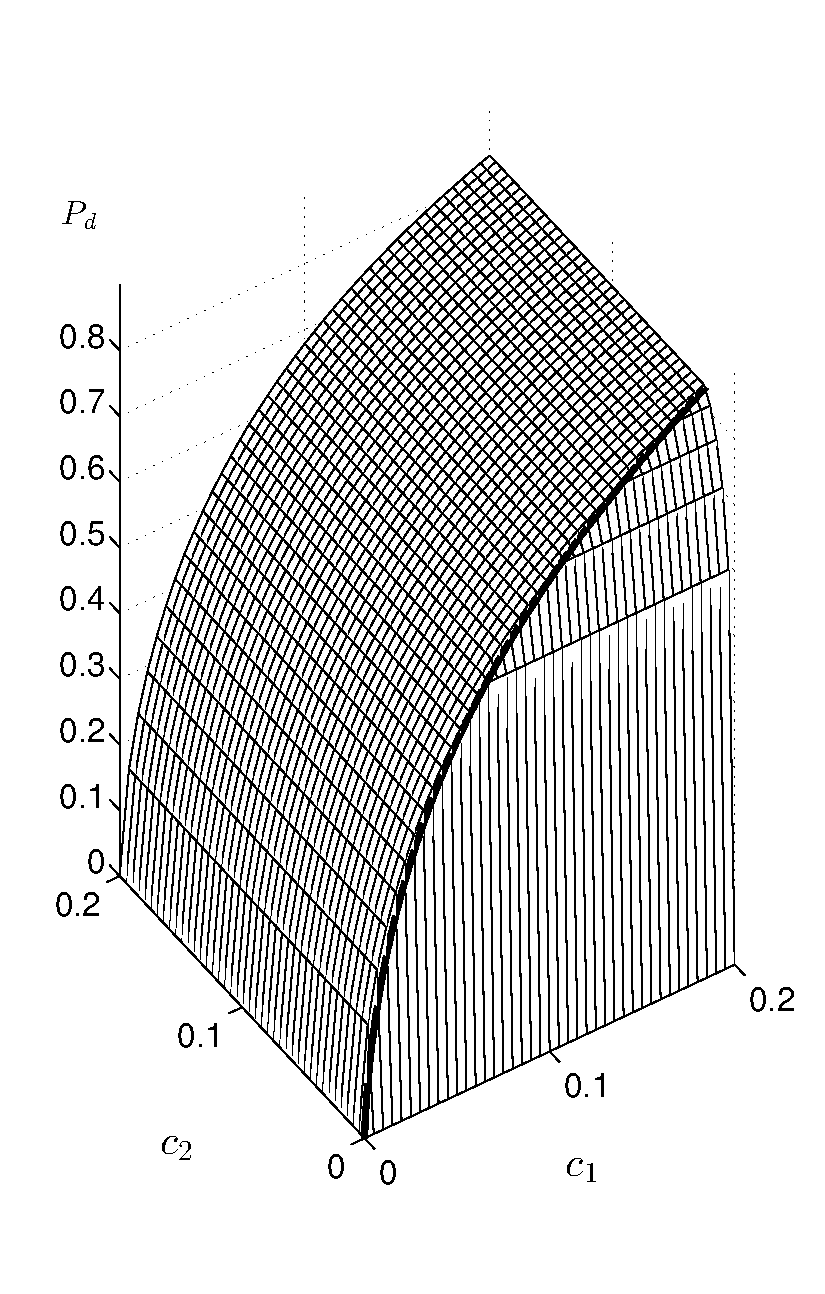
\includegraphics[width=12cm, height=16cm]{4/mathc1c2pd.eps}
\caption{M-ROC surface for $\sigma_n^2 = 0.1$, $\sigma_{s_A}^2=0.05$, $\sigma_{s_B}^2=0.15$ and $N = 20$.}
\label{pic:1201a1}
\end{figure}

\subsection{Simulation Results}
The simulation results presented in this thesis were obtained by using Monte Carlo techniques. All of Matlab code for the programs required to reproduce the simulation results are contained in the attached CD. Appendix B presents a brief tutorial on the uses of the various files for the simulation. The system model and parameters are the same with the numerical analysis.

The simulation presents the performance of energy detector when $c_1$ and $c_2$ separately increase from $0.005$ to $0.2$ with steps $0.005$. For a specified $c_1$ and $c_2$, we compute  its associated MENP decision rule, which is given by \eqref{equ:1129a4} and \eqref{equ:2015may1a2}. 

For each decision rule calculated through \eqref{equ:1129a4} and \eqref{equ:2015may1a2}, we use Monte Carlo simulation to get its associated $P_d$, $P_{f_1}$ and $P_{f_2}$.   
In order to ensure highly accurate results, a minimum of 600 events and 100000 experiments are required. The simulation result of the M-ROC surface is presented in Fig. \ref{pic:2015may1}. $P_d$ is acquired through simulation for each intersection of the mesh in Fig. \ref{pic:2015may1}, except for points $c_1 = 0$, $c_2$ and $c_2 = 0$, $c_1$, which are plotted to better illustrate the M-ROC surface. 
Compare Fig. \ref{pic:2015may1} with Fig. \ref{pic:1201a1}, we can see the simulation result accords with the numerical analysis, which verify our theoretical analysis.

Fig. \ref{pic:2015may1a0} depicts the relationship between  $P_d$ and $V_\tau$ for each $V_\tau$  computed through \eqref{equ:2015may1a2}.  For each $c_1, c_2$, the associated $(V_\tau, P_d)$ is plotted as `o'. The curve in Fig. \ref{pic:2015may1a1} is the theoretical relationship between $P_d$ and $V_\tau$ calculated through \eqref{equ:1129a5}. 
Since $c_1$ and $c_2$ are discrete, the value of $V_\tau$ is also discrete (as we can see from Fig. \ref{pic:2015may1a0}). Furthermore, for different $(c_1, c_2)$, the value of $V_\tau$ may be the same, 
e.g. for $(c_1, c_2) = (0.1, 0.1)$, the value of $V_\tau$ is $4.358$; for $(c_1, c_2) = (0.1, 0.2)$, we have $V_\tau = 4.358$.  
In our program, we use Monte Carlo simulations to acquire the $P_d$ for each $(c_1, c_2)$.  For  $(c_1, c_2) = (0.1, 0.1)$, the $P_d$ we acquired is $0.67819$; for $(c_1, c_2) = (0.1, 0.2)$, the $P_d$ we acquired through simulation is $0.67823$. There are some slight difference between the two $P_d$ (even though the decision rule are the same). This is because when the   experiments times is not unlimited, the simulation results could be different from the theoretical results. This explains why in Fig. \ref{pic:2015may1a0} for one $V_\tau$ value, there may be multiple $P_d$ corresponds with it.  
From Fig. \ref{pic:2015may1a0}, we can see the simulation result accords with the numerical analysis. 

Fig. \ref{pic:2015may1a1} depicts the relationship between $P_{f_1}$, $P_{f_2}$ and $P_d$ for each decision rule computed through \eqref{equ:2015may1a2}.  
For each $c_1, c_2$, the associated $(P_{f_1}, P_{f_2}, P_d) $ is plotted as `o'.
The curve in Fig. \ref{pic:2015may1a1} is the theoretical relationship between $P_{f_1}$ $P_{f_2}$ and $P_d$. This curve is computed through \eqref{equ: pd under x0}. 
As we have discussed, for one decision rule, there could be multiple simulation results for $(P_{f_1}, P_{f_2}, P_d)$, and these simulation results may be slight different due to the experiments times' limitation. 
This explains why in Fig. \ref{pic:2015may1a1} for some $(P_{f_1}, P_{f_2}, P_d)$ points, there are several  `o' around the theoretical curve.
By comparing the simulation results and the theoretical curve, we can see the simulation result accords with the numerical analysis. 


\begin{figure}[!t]
\centering
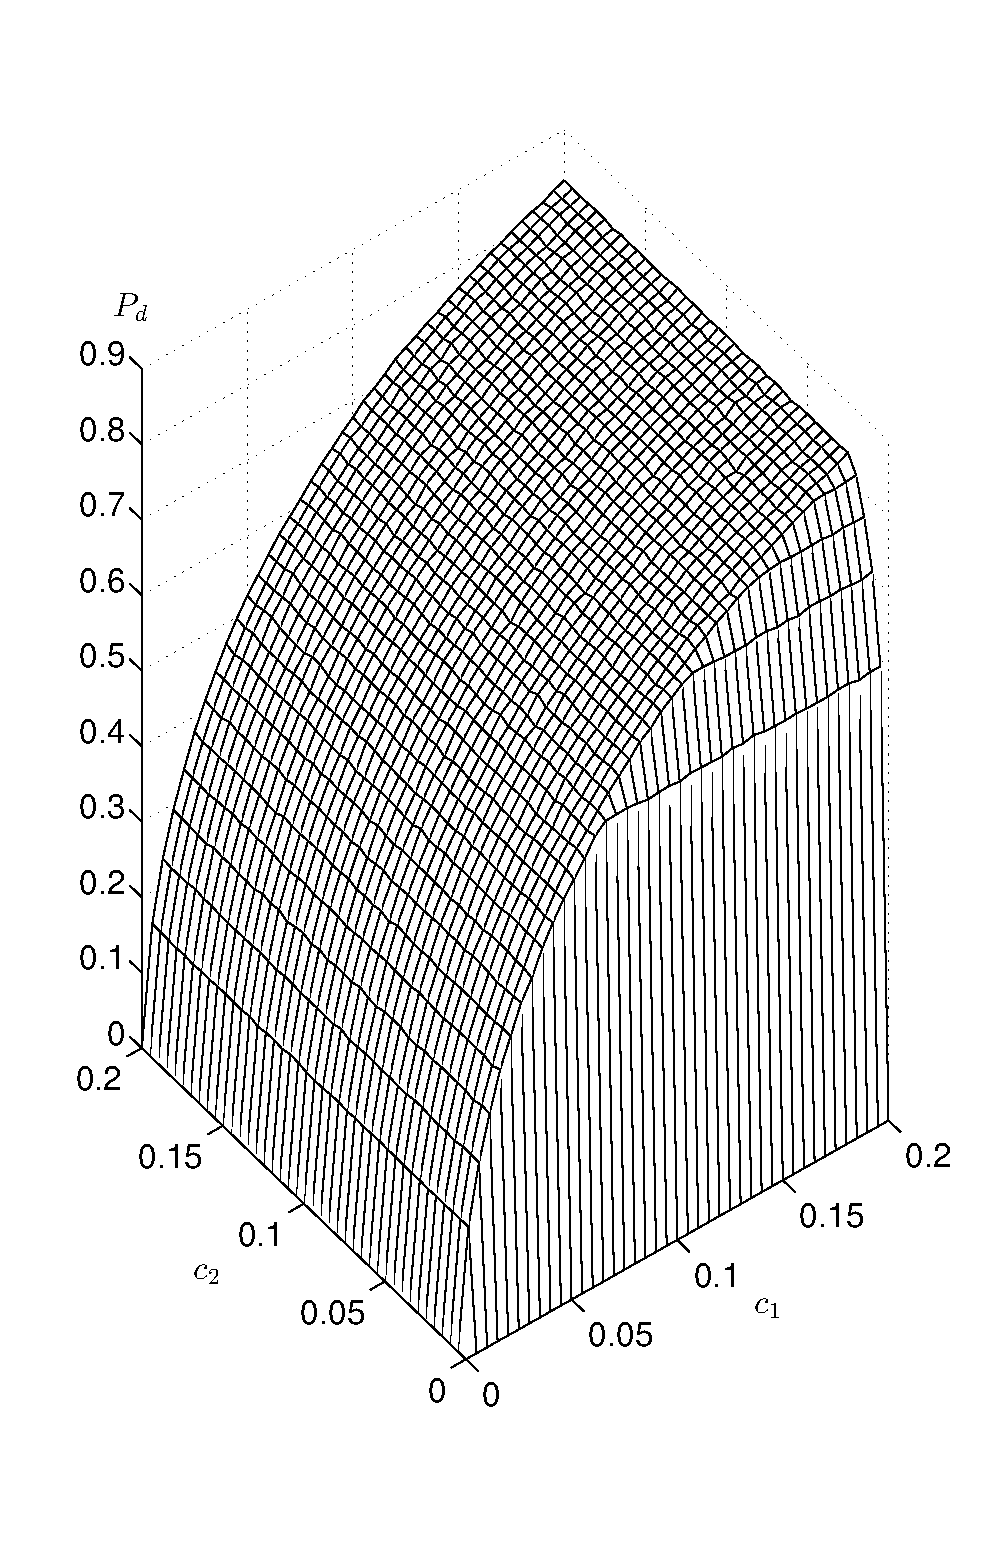
\includegraphics[width=12cm, height=16cm]{4/c1c2pd.eps}
\caption{Simulation results of M-ROC surface for $\sigma_n^2 = 0.1$, $\sigma_{s_A}^2=0.05$, $\sigma_{s_B}^2=0.15$ and $N = 20$.}
\label{pic:2015may1}
\end{figure}


\begin{figure}[!t]
\centering
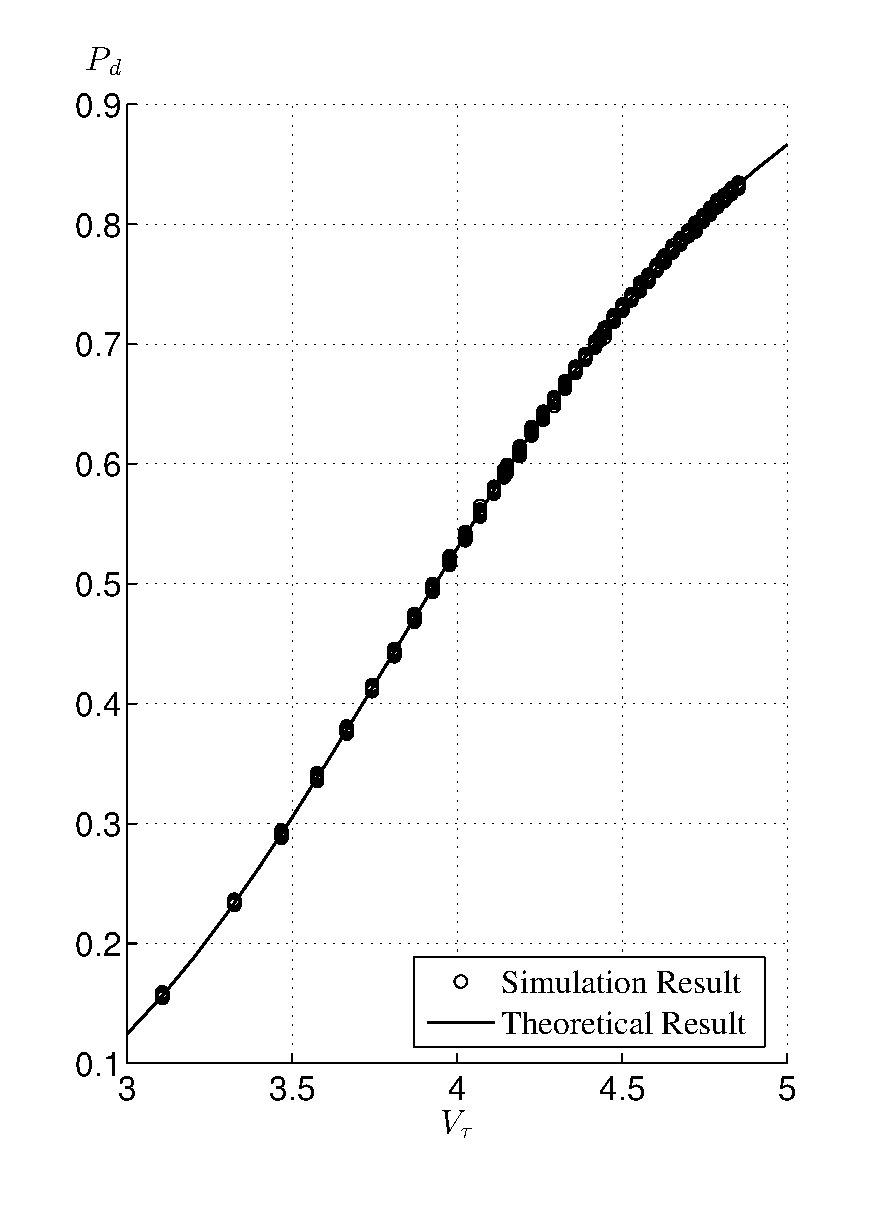
\includegraphics[width=12cm, height=16cm]{4/tpd.eps}
\caption{Relationship Between $V_\tau$ and its associated $P_d$.}
\label{pic:2015may1a0}
\end{figure}

\begin{figure}[!t]
\centering
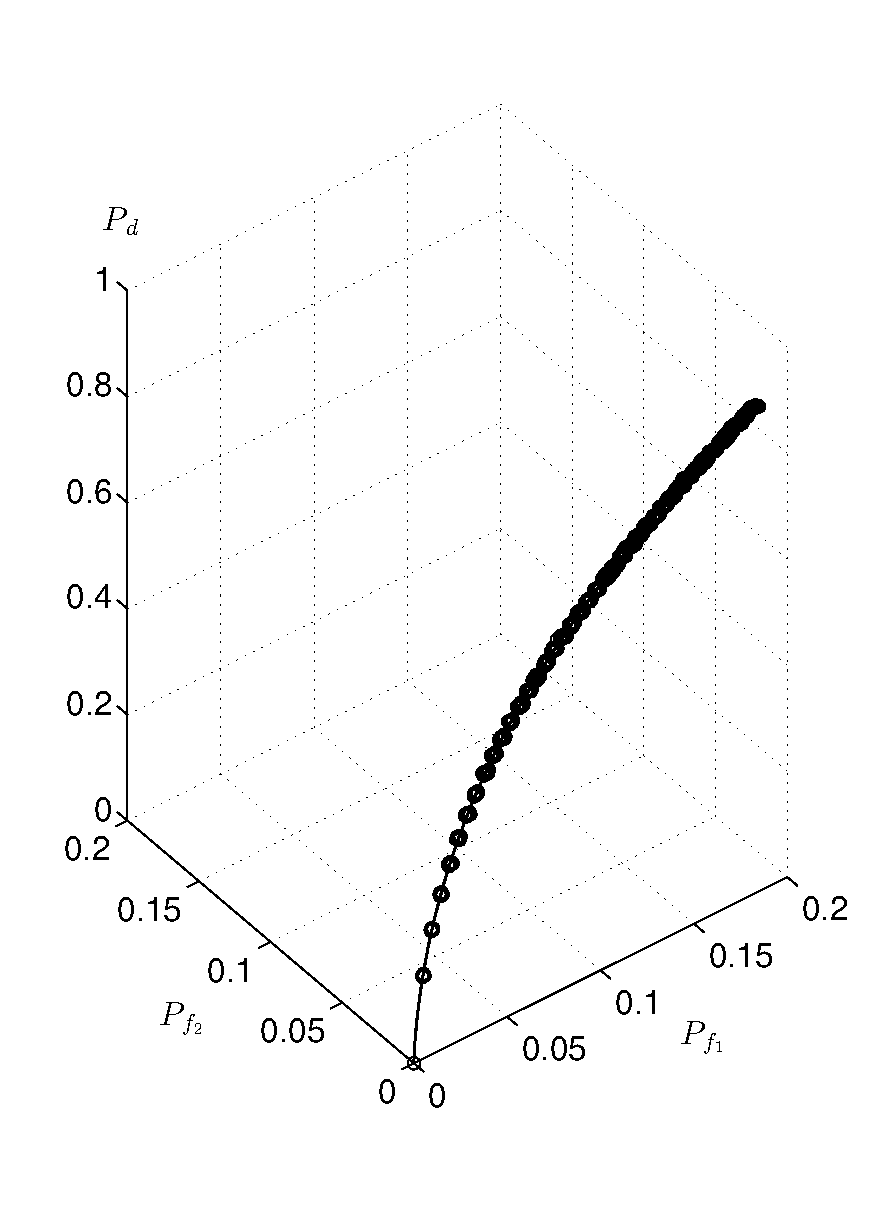
\includegraphics[width=12cm, height=16cm]{4/pdpf1pf2.eps}
\caption{Relationship between $P_{f_1}$, $P_{f_2}$ and $P_d$.}
\label{pic:2015may1a1}
\end{figure}



%----------------------------------------------------------------------------------------------


\typeout{}
% cyclostationary based energy detection
\section{Cyclostationary Detection for multiple Primary Users}
\subsection{System Model}

We consider a cognitive radio system where the spectrum can be occupied by exactly one of two distinct primary signals $\{s_A, s_B\}$ or it could be vacant. Let $H_0$ denote the situation under which the channel is free, $H_1$ denote the hypothesis under which the channel is occupied by signal $s_A$ and $H_2$ denote the hypothesis under which the channel is occupied by signals $s_B$. Both $s_A, s_B$ are OFDM signals with same frame structure. The block diagram of the system is illustrated in Figure.

\begin{figure}[!t]
  \centering 
  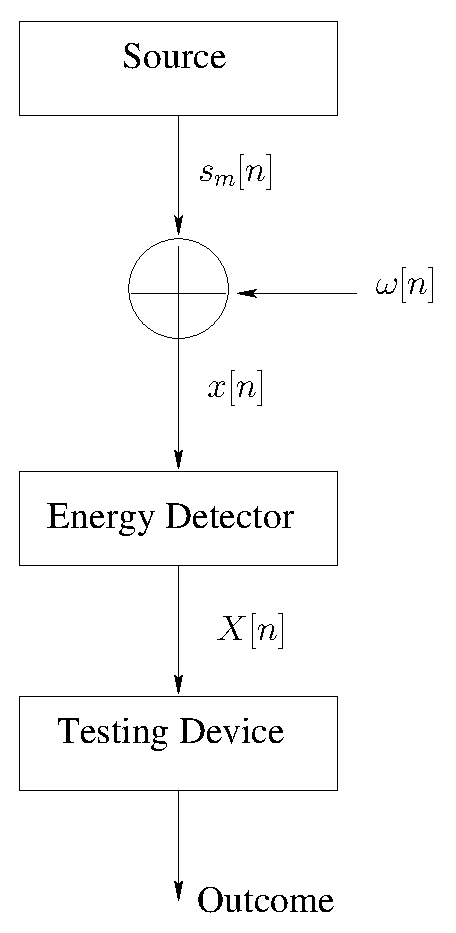
\includegraphics[width=\textwidth]{4/fig1.eps}
  \caption{Block Diagram for  cyclostationary detector.}
  \label{pic:1222a0}
\end{figure}
The measuring device observes $M$ samples of the noise version signals that could present in the channel and output a suitable testing statistics. With this statistics, the testing device employs MENP to determine the status of the channel. The input of measuring device is
\begin{equation}
  \mathbf{x} = \begin{cases}
	\mathbf{n}\;\;\;\;\;\;&\text{when $H_0$ is true}\\
	\mathbf{n}+\mathbf{s}_A\;\;\;\;\;\;&\text{when $H_1$ is true}\\
	\mathbf{n}+\mathbf{s}_B\;\;\;\;\;\;&\text{when $H_2$ is true}\\
  \end{cases}
  \label{equ:1209a1}
\end{equation}
where 
\begin{equation}
  \begin{cases}
	&\mathbf{x} = (x_0, x_1, \cdots, x_{M-1})\\
	&\mathbf{s}_A = (s_{A0}, s_{A1}, \cdots, s_{A(M-1)})\\
	&\mathbf{s}_B = (s_{B0}, s_{B1}, \cdots, s_{B(M-1)})\\
	&\mathbf{n} = (n_{0}, n_{1}, \cdots, n_{M-1})\,.
  \end{cases}
  \label{xssn}
\end{equation}
Assume each OFDM frame contains a CP sequence of length $l_C$ followed by a data sequence of length $l_D$, so the total length of an OFDM frame is $l_0 = l_C+l_D$. In general case, when there are signal transmitting, the receiver is not synchronized to the transmitted signal, i.e. $s_{A0}$ ( or $s_{B0}$) is not the first symbol of an OFDM frame. Let $\tau$ represents the synchronization mismatch. That is, when $\tau = 0$, $s_0$ is the first symbol of an OFDM frame; when $\tau = l_C+l_D -1$, $s_0$ is the last symbol of an OFDM frame. Let $M = Kl_0$, we can see when perfect synchronization the detector would observe $K$ complete  OFDM frames (as it is shown in Figure); otherwise, the detector would observe $K-1$ complete OFDM frames and $2$ incomplete OFDM frames (as it is shown in Figure). 
\begin{figure}[!t]
  \centering 
  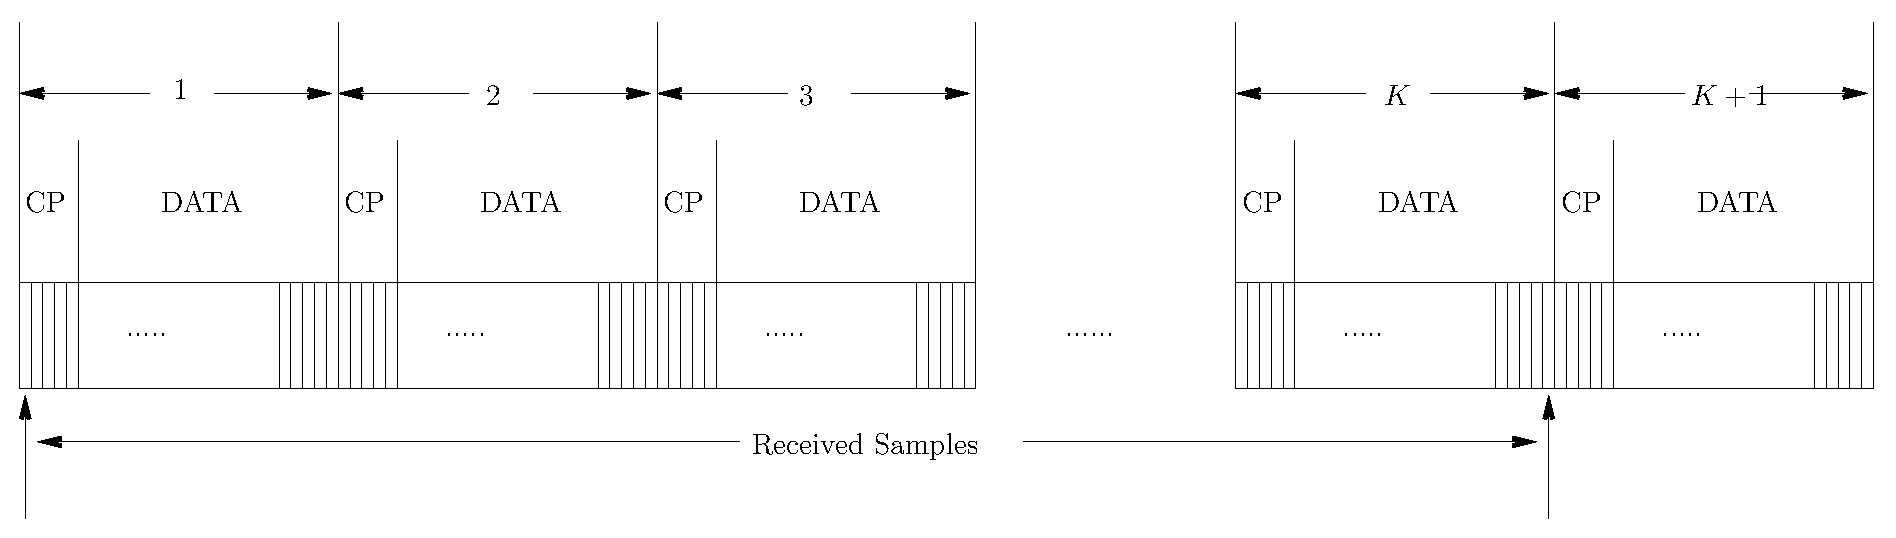
\includegraphics[width=\textwidth]{4/fig2.eps}
  \caption{Received signal for perfect synchronization.}
  \label{pic:1221n0}
\end{figure}

\begin{figure}[!t]
  \centering 
  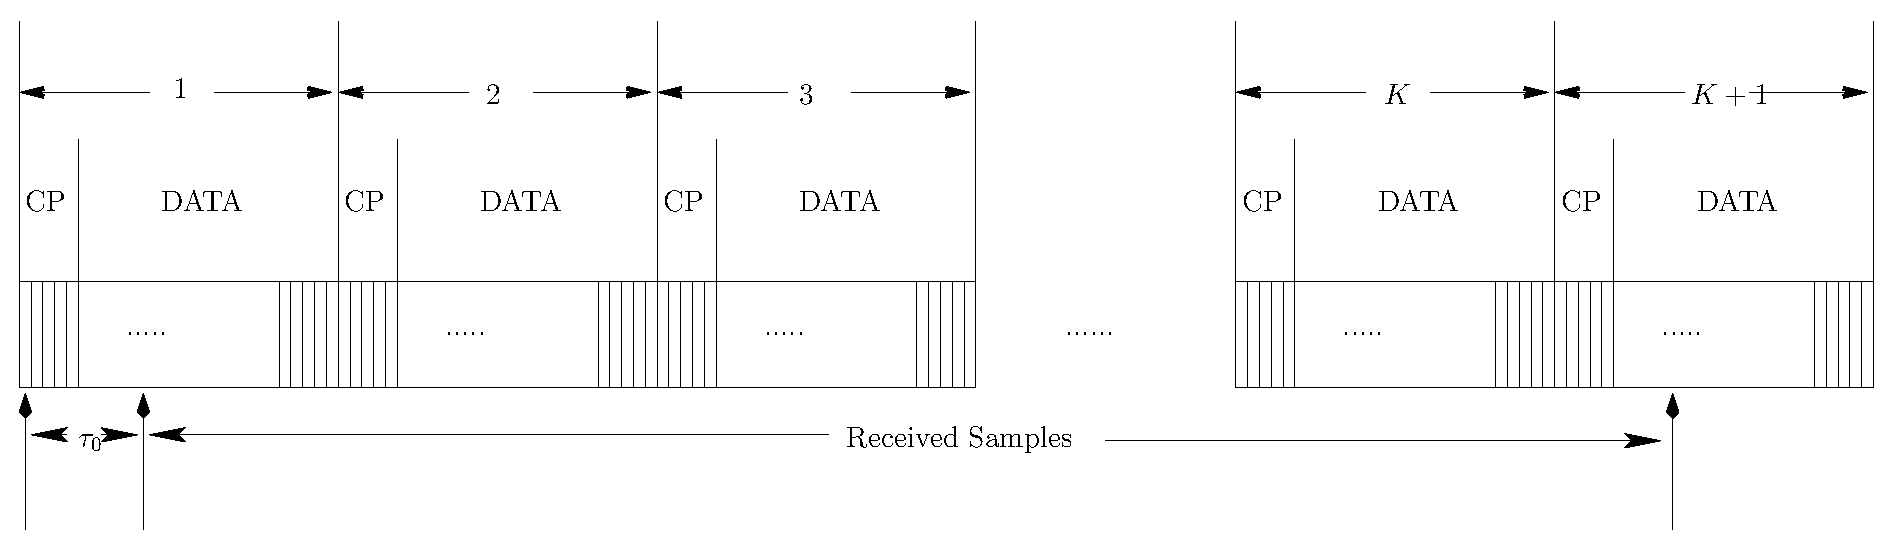
\includegraphics[width=\textwidth]{4/fig3.eps}
  \caption{Received signal for synchronization mismatch $\tau_0$.}
  \label{pic:1222a2}
\end{figure}
Assume $\tau = \tau_0$, let $\Theta_{\tau_0}$ denote the set of subscripts such that if $i \in \Theta_{\tau_0}$,  $s_i$ is a symbol of CP sequence. [To be added].
From Figure XX, we can see $i \in \Theta_{\tau_0}$ only if $i + \tau_0 \in [Ql_0, Ql_0+l_c -1]$ ($Q = 0, 1, \cdots, K-1$). 
Let $\Theta_{\tau_0}^k$ denotes set $\Theta_{\tau_0}$ subtract set $\{k\}$ ($k$ is also a subscript), i.e.
\begin{equation}
  \{i\in \Theta_{\tau_0}^k| i + \tau_0 \in [Ql_0, Ql_0+l_c -1] (Q = 0, 1, \cdots, K-1)\;\;\;\; \text{and}\;\;\;\; i\neq k\}
  \label{definitionof}
\end{equation}

Like in (c.f. ), we make following assumptions about the noise and signal: (1) all noise samples are i.i.d. mean zero circularly symmetric complex Gaussian (CSCG) with variance $\sigma_n^2$; (2) under hypothesis $H_1$ the transmitted signal symbols in the data sequence are i.i.d. zero mean CSCG with variance $\sigma_{s_A}^2$ (or $\sigma_{s_B}^2$ under hypothesis $H_2$); (3) if $s_i$ is a sample in CP sequence, then we have $s_i = s_{i+l_D}$. 

The CP structure could introduce strong cyclostationarity to the transmitted OFDM signals ($s_A$ or $s_B$) \cite{lunden2010robust}. 
Let $r_i=x_ix_j^\ast$ ($j=i+l_D$), \cite{lunden2007spectrum} shows $r_i$ exhibit cyclic property at frequency $\alpha = \frac{Q}{l_0}$ ($Q = \pm1, \pm2, \cdots$). In this case, we consider a single cyclic detector at frequency $\alpha = \frac{1}{l_0}$. 
Let $\mathbf{r}$ denote the vector of $r_i$, since the length of vector $\mathbf{x}$ is $M$, the length of $\mathbf{r}$ is $M - l_D$. For simple representation, let $N = M - l_D$.
Like in most related literature reviews (c.f. \cite{lunden2010robust} \cite{dandawate1994statistical}), the cyclic-covariance estimator for frequency $\alpha$ can be written as
\begin{equation}
  \hat{R}(l_D, \alpha) = \frac{1}{N}\sum_{i=0}^{N-1} r_ib_i\,.
  \label{cyclicR}
\end{equation}
where $b_i = \exp(-j2\pi\alpha i)$. 
The output of the measuring device is the real and imaginary part of the cyclic covariance estimator, i.e. 
\begin{equation}
  Y = \begin{bmatrix}
	R \\
	I
  \end{bmatrix}\,,
  \label{cyclic_cov}
\end{equation}
where 
\[
  R = \Re(\hat{R}(l_D, \alpha))
\]
and 
\[
  I = \Im(\hat{R}(l_D, \alpha))\,.
\]
By observing $y$, a realization  of $Y$, the testing device determines the status of the channel.
According to \cite{lunden2010robust}, $\hat{R}(l_D, \alpha)$ subjects to normal distribution for a large $K$, so $Y$ has the two-dimensional Gaussian distribution \cite{goodman1963statistical}.
Let $\bar{c}$ and $\tilde{c}$ denote the real and imaginary parts of a complex number $c$ respectively. Then, $b_i = \bar{b}_i + j\tilde{b}_i$  and $r_i = \bar{r}_i + j\tilde{r}_i$. 

The moment function of $\bar{r}_i, \tilde{r}_i$ are derived in \cite{axell2011optimal} and summarized in Table \ref{Table1} on page \pageref{Table1}.

% Please add the following required packages to your document preamble:
% \usepackage{multirow}
\begin{table}[h]
\centering
  \begin{tabular}{|c|c|c|c|c|c|}
	\hline
	\multirow{2}{*}{}           & \multirow{2}{*}{$H_0$} & \multicolumn{2}{c|}{$H_1$}                                                               & \multicolumn{2}{c|}{$H_2$}                                                               \\ \cline{3-6} 
	&                        & $i \in \Theta_{\tau_0}$                                                   & $i\notin \Theta_{\tau_0}$                          & $i\in \Theta_{\tau_0}$                                                   & $i\notin \Theta_{\tau_0}$                          \\ \hline
	$E[\bar{r}_i]$              & $0$                    & $2\sigma_{s_A}^2$                                       & $0$                            & $2\sigma_{s_B}^2$                                                         & $0$                            \\ \hline
	$E[\tilde{r}_i]$            & $0$                    & $0$                                                     & $0$                            & $0$                                                     & $0$                            \\ \hline
	$E[\bar{r}_i^2]$            & $2\sigma_n^4$          & $8\sigma_{s_A}^4+4\sigma_{s_A}^2\sigma_n^2+2\sigma_n^4$ & $2(\sigma_n^2+\sigma_{s_A}^2)^2$ & $8\sigma_{s_B}^4+4\sigma_{s_B}^2\sigma_n^2+2\sigma_n^4$ & $2(\sigma_n^2+\sigma_{s_B}^2)^2$ \\ \hline
	$E[\tilde{r}_i^2]$          & $2\sigma_n^4$          & $4\sigma_{s_A}^2\sigma_n^2+2\sigma_n^4$                 & $2(\sigma_n^2+\sigma_{s_A}^2)^2$ & $4\sigma_{s_B}^2\sigma_n^2+2\sigma_n^4$                 & $2(\sigma_n^2+\sigma_{s_B}^2)^2$ \\ \hline
	$E[\bar{r}_i\tilde{r}_i]$   & $0$                    & $0$                                                     & $0$                            & $0$                                                     & $0$                            \\ \hline
  \end{tabular}
  \caption{Moment function of $r_i$}
  \label{Table1}
\end{table}

Next we compute $E[\bar{r}_i\bar{r}_k]$, $E[\bar{r}_i\tilde{r}_k]$ and $E[\tilde{r}_i\tilde{r}_k]$ when $i \neq k$ under hypothesis $H_1$. For easy presentation, let $j = i+l_D$ and $l=k+l_D$.
 The expression of $r_i$ can be written as
\begin{equation}
  \begin{split}
    r_i = &(s_i+n_i)(s_j + n_j)^\ast\\
    = &(\bar{s}_i+j\tilde{s}_i + \bar{n}_i+j\tilde{n}_i)(\bar{s}_j-j\tilde{s}_j + \bar{n}_j-j\tilde{n}_j)\\
    = &\bar{s}_i\bar{s}_j + \bar{s}_i\bar{n}_j +\tilde{s}_i\tilde{s}_j+\tilde{s}_i\tilde{n}_j + \bar{n}_i\bar{s}_j+\bar{n}_i\bar{n}_j+\tilde{n}_i\tilde{s}_j+\tilde{n}_i\tilde{n}_j\\
    + &j\left( \tilde{s}_i\bar{s}_j + \tilde{s}_i\bar{n}_j + \tilde{n}_i\bar{s}_j + \tilde{n}_i\bar{n}_j - \bar{s}_i\tilde{s}_j - \bar{s}_i\tilde{n}_j - \bar{n}_i\tilde{s}_j - \bar{n}_i\tilde{n}_j \right)
  \end{split}
\end{equation}
thus we have 
\begin{equation}
  \begin{cases}
    \bar{r}_i = \bar{s}_i\bar{s}_j + \bar{s}_i\bar{n}_j +\tilde{s}_i\tilde{s}_j+\tilde{s}_i\tilde{n}_j + \bar{n}_i\bar{s}_j+\bar{n}_i\bar{n}_j+\tilde{n}_i\tilde{s}_j+\tilde{n}_i\tilde{n}_j\\
    \tilde{r}_i = \tilde{s}_i\bar{s}_j + \tilde{s}_i\bar{n}_j + \tilde{n}_i\bar{s}_j + \tilde{n}_i\bar{n}_j - \bar{s}_i\tilde{s}_j - \bar{s}_i\tilde{n}_j - \bar{n}_i\tilde{s}_j - \bar{n}_i\tilde{n}_j\,.
  \end{cases}
  \label{RrIr}
\end{equation}

\begin{equation}
  \begin{split}
    E[\bar{r}_i\bar{r}_k] = &E[(\bar{s}_i\bar{s}_j + \bar{s}_i\bar{n}_j +\tilde{s}_i\tilde{s}_j+\tilde{s}_i\tilde{n}_j + \bar{n}_i\bar{s}_j+\bar{n}_i\bar{n}_j+\tilde{n}_i\tilde{s}_j+\tilde{n}_i\tilde{n}_j)\\
    &(\bar{s}_k\bar{s}_l + \bar{s}_k\bar{n}_l +\tilde{s}_k\tilde{s}_l+\tilde{s}_k\tilde{n}_l + \bar{n}_k\bar{s}_l+\bar{n}_k\bar{n}_l+\tilde{n}_k\tilde{s}_l+\tilde{n}_k\tilde{n}_l)]\\
    = &E[\bar{s}_j\bar{s}_k\bar{s}_i\bar{s}_l]+E[\bar{s}_j\bar{s}_k\bar{s}_i\bar{n}_l]+E[\bar{s}_j\tilde{s}_k\bar{s}_i\tilde{s}_l]+E[\bar{s}_j\tilde{s}_k\bar{s}_i\tilde{n}_l]+E[\bar{s}_j\bar{n}_k\bar{s}_i\bar{s}_l]\\
&+E[\bar{s}_j\bar{n}_k\bar{s}_i\bar{n}_l]+E[\bar{s}_j\tilde{n}_k\bar{s}_i\tilde{s}_l]+E[\bar{s}_j\tilde{n}_k\bar{s}_i\tilde{n}_l]+E[\bar{n}_j\bar{s}_i\bar{s}_l\bar{s}_k]+E[\bar{n}_j\bar{s}_i\bar{n}_l\bar{s}_k]\\
&+E[\tilde{s}_k\bar{n}_j\bar{s}_i\tilde{s}_l]+E[\tilde{s}_k\bar{n}_j\bar{s}_i\tilde{n}_l]+E[\bar{n}_j\bar{n}_k\bar{s}_i\bar{s}_l]+E[\bar{n}_j\bar{n}_k\bar{s}_i\bar{n}_l]+E[\bar{n}_j\tilde{n}_k\bar{s}_i\tilde{s}_l]\\
&+E[\bar{n}_j\tilde{n}_k\bar{s}_i\tilde{n}_l]+E[\tilde{s}_j\tilde{s}_i\bar{s}_l\bar{s}_k]+E[\tilde{s}_j\tilde{s}_i\bar{n}_l\bar{s}_k]+E[\tilde{s}_k\tilde{s}_j\tilde{s}_i\tilde{s}_l]+E[\tilde{s}_k\tilde{s}_j\tilde{s}_i\tilde{n}_l]\\
&+E[\tilde{s}_j\tilde{s}_i\bar{n}_k\bar{s}_l]+E[\tilde{s}_j\tilde{s}_i\bar{n}_k\bar{n}_l]+E[\tilde{s}_j\tilde{s}_i\tilde{n}_k\tilde{s}_l]+E[\tilde{s}_j\tilde{s}_i\tilde{n}_k\tilde{n}_l]+E[\bar{s}_k\tilde{s}_i\tilde{n}_j\bar{s}_l]\\
&+E[\bar{s}_k\tilde{s}_i\tilde{n}_j\bar{n}_l]+E[\tilde{s}_k\tilde{s}_i\tilde{n}_j\tilde{s}_l]+E[\tilde{s}_k\tilde{s}_i\tilde{n}_l\tilde{n}_j]+E[\tilde{s}_i\bar{n}_k\tilde{n}_j\bar{s}_l]+E[\tilde{s}_i\bar{n}_k\tilde{n}_j\bar{n}_l]\\
&+E[\tilde{s}_i\tilde{n}_k\tilde{n}_j\tilde{s}_l]+E[\tilde{s}_i\tilde{n}_k\tilde{n}_l\tilde{n}_j]+E[\bar{n}_i\bar{s}_j\bar{s}_l\bar{s}_k]+E[\bar{n}_i\bar{s}_j\bar{n}_l\bar{s}_k]+E[\bar{n}_i\bar{s}_j\tilde{s}_k\tilde{s}_l]\\
&+E[\bar{n}_i\bar{s}_j\tilde{n}_l\tilde{s}_k]+E[\bar{n}_i\bar{s}_j\bar{n}_k\bar{s}_l]+E[\bar{n}_i\bar{s}_j\bar{n}_k\bar{n}_l]+E[\bar{n}_i\bar{s}_j\tilde{n}_k\tilde{s}_l]+E[\bar{n}_i\bar{s}_j\tilde{n}_k\tilde{n}_l]\\
&+E[\bar{n}_i\bar{s}_k\bar{n}_j\bar{s}_l]+E[\bar{n}_i\bar{s}_k\bar{n}_j\bar{n}_l]+E[\bar{n}_i\tilde{s}_k\bar{n}_j\tilde{s}_l]+E[\bar{n}_i\tilde{s}_k\bar{n}_j\tilde{n}_l]+E[\bar{n}_i\bar{n}_k\bar{n}_j\bar{s}_l]\\
&+E[\bar{n}_i\bar{n}_k\bar{n}_j\bar{n}_l]+E[\bar{n}_i\tilde{n}_k\bar{n}_j\tilde{s}_l]+E[\bar{n}_i\tilde{n}_k\bar{n}_j\tilde{n}_l]+E[\tilde{n}_i\bar{s}_k\bar{s}_l\tilde{s}_j]+E[\tilde{n}_i\bar{n}_l\bar{s}_k\tilde{s}_j]\\
&+E[\tilde{s}_k\tilde{n}_i\tilde{s}_l\tilde{s}_j]+E[\tilde{s}_k\tilde{n}_i\tilde{n}_l\tilde{s}_j]+E[\tilde{n}_i\bar{n}_k\bar{s}_l\tilde{s}_j]+E[\tilde{n}_i\bar{n}_k\bar{n}_l\tilde{s}_j]+E[\tilde{s}_l\tilde{n}_i\tilde{n}_k\tilde{s}_j]\\
&+E[\tilde{n}_i\tilde{n}_k\tilde{n}_l\tilde{s}_j]+E[\tilde{n}_i\tilde{n}_j\bar{s}_l\bar{s}_k]+E[\tilde{n}_i\tilde{n}_j\bar{n}_l\bar{s}_k]+E[\tilde{s}_k\tilde{n}_i\tilde{n}_j\tilde{s}_l]+E[\tilde{s}_k\tilde{n}_i\tilde{n}_j\tilde{n}_l]\\
&+E[\tilde{n}_i\tilde{n}_j\bar{n}_k\bar{s}_l]+E[\tilde{n}_i\tilde{n}_j\bar{n}_k\bar{n}_l]+E[\tilde{n}_i\tilde{n}_j\tilde{n}_k\tilde{s}_l]+E[\tilde{n}_i\tilde{n}_j\tilde{n}_k\tilde{n}_l]
  \end{split}
  \label{Erij}
\end{equation}
Since noise samples are governed by i.i.d Gaussian distribution with zero mean and they are independent with signals, items in \eqref{Erij} containing noise samples would have zero value, e.g. $E[\bar{s}_j\bar{s}_k\bar{s}_i\bar{n}_l] = E[\bar{s}_j\bar{s}_k\bar{s}_i]E[\bar{n}_l] = 0$. Eliminate zero value items in equation \eqref{Erij}:
\begin{equation}
  E[\bar{r}_i\bar{r}_k] = E[\bar{s}_i\bar{s}_j\bar{s}_k\bar{s}_l] + E[\bar{s}_i\bar{s}_j\tilde{s}_k\tilde{s}_l] + E[\tilde{s}_i\tilde{s}_j\bar{s}_k\bar{s}_l] + E[\tilde{s}_i\tilde{s}_j\tilde{s}_k\tilde{s}_l]
  \label{equ:Erirk}
\end{equation} 

Without losing generality, we assume $i < k$. Consider the situation when $k \notin \Theta_{\tau_0}$, in such case $s_k$ and $s_l$ are independent. It is easy to see $s_l$ is also independent with $s_i$ and $s_j$. Hence \eqref{equ:Erirk} can be written as
\begin{equation}
  \begin{split}
  E[\bar{r}_i\bar{r}_k] = &E[\bar{s}_i\bar{s}_j\bar{s}_k]E[\bar{s}_l] + E[\bar{s}_i\bar{s}_j\tilde{s}_k]E[\tilde{s}_l] + E[\tilde{s}_i\tilde{s}_j\bar{s}_k]E[\bar{s}_l] + E[\tilde{s}_i\tilde{s}_j\tilde{s}_k]E[\tilde{s}_l]\\
  = &0\,.
\end{split}
  \label{equ:Erirksitu1}
\end{equation} 
Similarly it can be proved when $i \notin \Theta_{\tau_0}$, we have $E[\bar{r}_i\bar{r}_k] =0$. Now consider the situation when $i, k \in \Theta_{\tau_0}$. In such case, we have 
\begin{equation}
  \begin{cases}
    s_i = s_j\\
    s_k = s_l
  \end{cases}
\end{equation}
and \eqref{equ:Erirk} can be written in form of
\begin{equation}
  \begin{split}
    E[\bar{r}_i\bar{r}_k] &= E[\bar{s}_i^2\bar{s}_k^2] + E[\bar{s}_i^2\tilde{s}_k^2]  +E[\tilde{s}_i^2\bar{s}_k^2] + E[\tilde{s}_i^2\tilde{s}_k^2] \\
    &= E[\bar{s}_i^2]E[\bar{s}_k^2] + E[\bar{s}_i^2]E[\tilde{s}_k^2]  +E[\tilde{s}_i^2]E[\bar{s}_k^2] + E[\tilde{s}_i^2]E[\tilde{s}_k^2] \\
    &= 4\sigma_{s_A}^4\,.
  \end{split}
  \label{Eririsitu2}
\end{equation}

From above discussion, the value of $E[\bar{r}_i\bar{r}_k]$  ($i \neq k$) can be summarized as
\begin{equation}
  E[\bar{r}_i\bar{r}_k] =  \begin{cases}
    4\sigma_{s_A}^4 \;\;\;\;&i, k \in \Theta_{\tau_0}\\
    0\;\;\;\;&\text{Otherwise}
  \end{cases}
  \label{Er_ir_j}
\end{equation}

Next consider $E[\bar{r}_i\tilde{r}_j]$, which can be written as
\begin{equation}
  \begin{split}
E[\bar{r}_i\tilde{r}_j] = &E[(\bar{s}_i\bar{s}_j + \bar{s}_i\bar{n}_j +\tilde{s}_i\tilde{s}_j+\tilde{n}_i\tilde{n}_j + \bar{n}_i\bar{s}_j+\bar{n}_i\bar{n}_j+\tilde{n}_i\tilde{s}_j+\tilde{n}_i\tilde{n}_j)\\
              &(\tilde{s}_k\bar{s}_l + \tilde{s}_k\bar{n}_l + \tilde{n}_k\bar{s}_l + \tilde{n}_k\bar{n}_l - \bar{s}_k\tilde{s}_l - \bar{s}_k\tilde{n}_l - \bar{n}_k\tilde{s}_l - \bar{n}_k\tilde{n}_l)]\,.
%              = &E[\bar{s}_j\tilde{s}_k\bar{s}_i\bar{s}_l]+E[\bar{s}_j\tilde{s}_k\bar{s}_i\bar{n}_l]+E[\bar{s}_j\tilde{n}_k\bar{s}_i\bar{s}_l]+E[\bar{s}_j\tilde{n}_k\bar{s}_i\bar{n}_l]-E[\bar{s}_j\bar{s}_k\bar{s}_i\tilde{s}_l]\\
%&-E[\bar{s}_j\bar{s}_k\bar{s}_i\tilde{n}_l]-E[\bar{s}_j\bar{n}_k\bar{s}_i\tilde{s}_l]-E[\bar{s}_j\bar{n}_k\bar{s}_i\tilde{n}_l]+E[\tilde{s}_k\bar{n}_j\bar{s}_i\bar{s}_l]+E[\tilde{s}_k\bar{n}_j\bar{s}_i\bar{n}_l]\\
%&+E[\bar{n}_j\tilde{n}_k\bar{s}_i\bar{s}_l]+E[\bar{n}_j\tilde{n}_k\bar{s}_i\bar{n}_l]-E[\tilde{s}_l\bar{n}_j\bar{s}_i\bar{s}_k]-E[\bar{n}_j\bar{s}_i\tilde{n}_l\bar{s}_k]-E[\bar{n}_j\bar{n}_k\bar{s}_i\tilde{s}_l]\\
%&-E[\bar{n}_j\bar{n}_k\bar{s}_i\tilde{n}_l]+E[\tilde{s}_k\tilde{s}_j\tilde{s}_i\bar{s}_l]+E[\tilde{s}_k\tilde{s}_j\tilde{s}_i\bar{n}_l]+E[\tilde{s}_j\tilde{s}_i\tilde{n}_k\bar{s}_l]+E[\tilde{s}_j\tilde{s}_i\tilde{n}_k\bar{n}_l]\\
%&-E[\tilde{s}_j\tilde{s}_i\tilde{s}_l\bar{s}_k]-E[\tilde{s}_j\tilde{s}_i\tilde{n}_l\bar{s}_k]-E[\tilde{s}_j\tilde{s}_i\bar{n}_k\tilde{s}_l]-E[\tilde{s}_j\tilde{s}_i\tilde{n}_l\bar{n}_k]+E[\tilde{s}_k\tilde{n}_i\tilde{n}_j\bar{s}_l]\\
%&+E[\tilde{s}_k\tilde{n}_i\tilde{n}_j\bar{n}_l]+E[\tilde{n}_i\tilde{n}_j\tilde{n}_k\bar{s}_l]+E[\tilde{n}_i\tilde{n}_j\tilde{n}_k\bar{n}_l]-E[\tilde{n}_i\tilde{n}_j\tilde{s}_l\bar{s}_k]-E[\tilde{n}_i\tilde{n}_j\tilde{n}_l\bar{s}_k]\\
%&-E[\tilde{n}_i\tilde{n}_j\bar{n}_k\tilde{s}_l]-E[\tilde{n}_i\tilde{n}_j\tilde{n}_l\bar{n}_k]+E[\bar{n}_i\bar{s}_j\bar{s}_l\tilde{s}_k]+E[\bar{n}_i\bar{s}_j\bar{n}_l\tilde{s}_k]+E[\bar{n}_i\bar{s}_j\tilde{n}_k\bar{s}_l]\\
%&+E[\bar{n}_i\bar{s}_j\tilde{n}_k\bar{n}_l]-E[\bar{n}_i\bar{s}_j\tilde{s}_l\bar{s}_k]-E[\bar{n}_i\bar{s}_j\tilde{n}_l\bar{s}_k]-E[\bar{n}_i\bar{s}_j\bar{n}_k\tilde{s}_l]-E[\bar{n}_i\bar{s}_j\bar{n}_k\tilde{n}_l]\\
%&+E[\bar{n}_i\tilde{s}_k\bar{n}_j\bar{s}_l]+E[\bar{n}_i\tilde{s}_k\bar{n}_j\bar{n}_l]+E[\bar{n}_i\tilde{n}_k\bar{n}_j\bar{s}_l]+E[\bar{n}_i\tilde{n}_k\bar{n}_j\bar{n}_l]-E[\bar{n}_i\bar{s}_k\bar{n}_j\tilde{s}_l]\\
%&-E[\bar{n}_i\bar{s}_k\bar{n}_j\tilde{n}_l]-E[\bar{n}_i\bar{n}_k\bar{n}_j\tilde{s}_l]-E[\bar{n}_i\bar{n}_k\bar{n}_j\tilde{n}_l]+E[\tilde{s}_k\tilde{n}_i\bar{s}_l\tilde{s}_j]+E[\tilde{s}_k\tilde{n}_i\bar{n}_l\tilde{s}_j]\\
%&+E[\tilde{n}_i\tilde{n}_k\bar{s}_l\tilde{s}_j]+E[\tilde{n}_i\tilde{n}_k\bar{n}_l\tilde{s}_j]-E[\tilde{n}_i\tilde{s}_l\bar{s}_k\tilde{s}_j]-E[\tilde{n}_i\tilde{n}_l\bar{s}_k\tilde{s}_j]-E[\tilde{n}_i\bar{n}_k\tilde{s}_l\tilde{s}_j]\\
%&-E[\tilde{n}_i\bar{n}_k\tilde{n}_l\tilde{s}_j]+E[\tilde{s}_k\tilde{n}_i\tilde{n}_j\bar{s}_l]+E[\tilde{s}_k\tilde{n}_i\tilde{n}_j\bar{n}_l]+E[\tilde{n}_i\tilde{n}_j\tilde{n}_k\bar{s}_l]+E[\tilde{n}_i\tilde{n}_j\tilde{n}_k\bar{n}_l]\\
%&-E[\tilde{n}_i\tilde{n}_j\tilde{s}_l\bar{s}_k]-E[\tilde{n}_i\tilde{n}_j\tilde{n}_l\bar{s}_k]-E[\tilde{n}_i\tilde{n}_j\bar{n}_k\tilde{s}_l]-E[\tilde{n}_i\tilde{n}_j\tilde{n}_l\bar{n}_k]
\end{split}
\label{Eriiiirk}
\end{equation}
expand \eqref{Eriiiirk} and eliminate zero value items (items including noise samples), we have 
 \begin{equation}
   E[\bar{r}_i\tilde{r}_k] = E[\bar{s}_j\tilde{s}_k\bar{s}_i\bar{s}_l] -  E[\bar{s}_j\bar{s}_k\bar{s}_i\tilde{s}_l] + E[\tilde{s}_j\tilde{s}_k\tilde{s}_i\bar{s}_l] - E[\tilde{s}_j\bar{s}_k\tilde{s}_i\tilde{s}_l]\,.
   \label{equ:1213a}
\end{equation}
Since the real and imaginary part of transmitted OFDM signals are independent and $E[\bar{s}_m] = E[\tilde{s}_m] = 0$ ($m = 0, 1, \cdots, N$), \eqref{equ:1213a} can be written as
\begin{equation}
  \begin{split}
  E[\bar{r}_i\tilde{r}_k] &= E[\tilde{s}_k]E[\bar{s}_i\bar{s}_j\bar{s}_l]  - E[\tilde{s}_l]E[\bar{s}_i\bar{s}_j\bar{s}_k] + E[\bar{s}_l]E[\tilde{s}_i\tilde{s}_j\tilde{s}_k] -  E[\bar{s}_k]E[\tilde{s}_i\tilde{s}_j\tilde{s}_l]\\
  &= 0
\end{split}
  \label{equ:1215m}
\end{equation}
thus we can see $E[\bar{r}_i\tilde{r}_k] = 0$  when $i \neq k $.  

Next consider $E[\tilde{r}_i\tilde{r}_k]$, which can be written as
\begin{equation}
  \begin{split}
    E[\tilde{r}_i\tilde{r}_k] = &E[(\tilde{s}_i\bar{s}_j + \tilde{s}_i\bar{n}_j + \tilde{n}_i\bar{s}_j + \tilde{n}_i\bar{n}_j - \bar{s}_i\tilde{s}_j - \bar{s}_i\tilde{n}_j - \bar{n}_i\tilde{s}_j - \bar{n}_i\tilde{n}_j)\\
    &(\tilde{s}_k\bar{s}_l + \tilde{s}_k\bar{n}_l + \tilde{n}_k\bar{s}_l + \tilde{n}_k\bar{n}_l - \bar{s}_k\tilde{s}_l - \bar{s}_k\tilde{n}_l - \bar{n}_k\tilde{s}_l - \bar{n}_k\tilde{n}_l)]
%    = &E[\bar{s}_j\tilde{s}_k\tilde{s}_i\bar{s}_l]+E[\bar{s}_j\tilde{s}_k\tilde{s}_i\bar{n}_l]+E[\bar{s}_j\tilde{s}_i\tilde{n}_k\bar{s}_l]+E[\bar{s}_j\tilde{s}_i\tilde{n}_k\bar{n}_l]-E[\bar{s}_j\bar{s}_k\tilde{s}_i\tilde{s}_l]\\
%&-E[\bar{s}_j\bar{s}_k\tilde{s}_i\tilde{n}_l]-E[\bar{s}_j\tilde{s}_i\bar{n}_k\tilde{s}_l]-E[\bar{s}_j\tilde{s}_i\tilde{n}_l\bar{n}_k]+E[\tilde{s}_k\tilde{s}_i\bar{n}_j\bar{s}_l]+E[\tilde{s}_k\tilde{s}_i\bar{n}_j\bar{n}_l]\\
%&+E[\tilde{n}_k\tilde{s}_i\bar{n}_j\bar{s}_l]+E[\tilde{n}_k\tilde{s}_i\bar{n}_j\bar{n}_l]-E[\bar{s}_k\tilde{s}_i\bar{n}_j\tilde{s}_l]-E[\bar{s}_k\tilde{s}_i\bar{n}_j\tilde{n}_l]-E[\tilde{s}_i\bar{n}_j\bar{n}_k\tilde{s}_l]\\
%&-E[\tilde{s}_i\bar{n}_j\tilde{n}_l\bar{n}_k]+E[\bar{s}_j\tilde{n}_i\bar{s}_l\tilde{s}_k]+E[\bar{s}_j\tilde{n}_i\bar{n}_l\tilde{s}_k]+E[\bar{s}_j\tilde{n}_i\tilde{n}_k\bar{s}_l]+E[\bar{s}_j\tilde{n}_i\tilde{n}_k\bar{n}_l]\\
%&-E[\bar{s}_j\tilde{n}_i\tilde{s}_l\bar{s}_k]-E[\bar{s}_j\tilde{n}_i\tilde{n}_l\bar{s}_k]-E[\bar{s}_j\tilde{n}_i\bar{n}_k\tilde{s}_l]-E[\bar{s}_j\tilde{n}_i\bar{n}_k\tilde{n}_l]+E[\tilde{s}_k\tilde{n}_i\bar{n}_j\bar{s}_l]\\
%&+E[\tilde{s}_k\tilde{n}_i\bar{n}_j\bar{n}_l]+E[\tilde{n}_i\tilde{n}_k\bar{n}_j\bar{s}_l]+E[\tilde{n}_i\tilde{n}_k\bar{n}_j\bar{n}_l]-E[\tilde{s}_l\tilde{n}_i\bar{n}_j\bar{s}_k]-E[\tilde{n}_i\bar{n}_j\tilde{n}_l\bar{s}_k]\\
%&-E[\tilde{n}_i\bar{n}_k\bar{n}_j\tilde{s}_l]-E[\tilde{n}_i\bar{n}_k\bar{n}_j\tilde{n}_l]-E[\tilde{s}_k\tilde{s}_j\bar{s}_i\bar{s}_l]-E[\tilde{s}_k\tilde{s}_j\bar{s}_i\bar{n}_l]-E[\tilde{s}_j\tilde{n}_k\bar{s}_i\bar{s}_l]\\
%&-E[\tilde{s}_j\tilde{n}_k\bar{s}_i\bar{n}_l]+E[\tilde{s}_l\tilde{s}_j\bar{s}_i\bar{s}_k]+E[\tilde{s}_j\bar{s}_i\tilde{n}_l\bar{s}_k]+E[\tilde{s}_j\bar{n}_k\bar{s}_i\tilde{s}_l]+E[\tilde{s}_j\bar{n}_k\bar{s}_i\tilde{n}_l]\\
%&-E[\tilde{s}_k\tilde{n}_j\bar{s}_i\bar{s}_l]-E[\tilde{s}_k\tilde{n}_j\bar{s}_i\bar{n}_l]-E[\tilde{n}_k\tilde{n}_j\bar{s}_i\bar{s}_l]-E[\tilde{n}_k\tilde{n}_j\bar{s}_i\bar{n}_l]+E[\bar{s}_k\tilde{n}_j\bar{s}_i\tilde{s}_l]\\
%&+E[\bar{s}_k\tilde{n}_j\bar{s}_i\tilde{n}_l]+E[\tilde{n}_j\bar{s}_i\bar{n}_k\tilde{s}_l]+E[\tilde{n}_j\bar{s}_i\tilde{n}_l\bar{n}_k]-E[\bar{n}_i\tilde{s}_j\bar{s}_l\tilde{s}_k]-E[\bar{n}_i\tilde{s}_j\bar{n}_l\tilde{s}_k]\\
%&-E[\bar{n}_i\tilde{s}_j\tilde{n}_k\bar{s}_l]-E[\bar{n}_i\tilde{s}_j\tilde{n}_k\bar{n}_l]+E[\bar{n}_i\tilde{s}_j\tilde{s}_l\bar{s}_k]+E[\bar{n}_i\tilde{s}_j\tilde{n}_l\bar{s}_k]+E[\bar{n}_i\tilde{s}_j\bar{n}_k\tilde{s}_l]\\
%&+E[\bar{n}_i\tilde{s}_j\bar{n}_k\tilde{n}_l]-E[\bar{n}_i\tilde{s}_k\tilde{n}_j\bar{s}_l]-E[\bar{n}_i\tilde{s}_k\tilde{n}_j\bar{n}_l]-E[\bar{n}_i\tilde{n}_j\tilde{n}_k\bar{s}_l]-E[\bar{n}_i\tilde{n}_j\tilde{n}_k\bar{n}_l]\\
%&+E[\bar{n}_i\bar{s}_k\tilde{n}_j\tilde{s}_l]+E[\bar{n}_i\bar{s}_k\tilde{n}_j\tilde{n}_l]+E[\bar{n}_i\tilde{n}_j\bar{n}_k\tilde{s}_l]+E[\bar{n}_i\tilde{n}_j\tilde{n}_l\bar{n}_k]
  \end{split}
  \label{EEEErrrrr}
\end{equation}
expand \eqref{EEEErrrrr} and eliminate zero value items (items including noise samples), we have 
\begin{equation}
  E[\tilde{r}_i\tilde{r}_k] = E[\bar{s}_j\tilde{s}_k\tilde{s}_i\bar{s}_l] -  E[\bar{s}_j\bar{s}_k\tilde{s}_i\tilde{s}_l] - E[\tilde{s}_j\tilde{s}_k\bar{s}_i\bar{s}_l] +E[\tilde{s}_j\bar{s}_k\bar{s}_i\tilde{s}_l]
  \label{1213night}
\end{equation}

Similar with $E[\bar{r}_i\bar{r}_k]$, when $i$ (or $k$) does not belong to set $\Theta_{\tau_0}$, we can see
$   E[\tilde{r}_i\tilde{r}_k] = 0$.

When $i, k \in \Theta_{\tau_0}$, equation \eqref{1213night} can be written as
\begin{equation}
  \begin{split}
  E[\tilde{r}_i\tilde{r}_k] = &E[\bar{s}_i\tilde{s}_k\tilde{s}_i\bar{s}_k] -  E[\bar{s}_i\bar{s}_k\tilde{s}_i\tilde{s}_k] - E[\tilde{s}_i\tilde{s}_k\bar{s}_i\bar{s}_k] +E[\tilde{s}_i\bar{s}_k\bar{s}_i\tilde{s}_k]\\
  = &E[\bar{s}_i]E[\tilde{s}_k]E[\tilde{s}_i]E[\bar{s}_k] -  E[\bar{s}_i]E[\bar{s}_k]E[\tilde{s}_i]E[\tilde{s}_k] - E[\tilde{s}_i]E[\tilde{s}_k]E[\bar{s}_i]E[\bar{s}_k] +E[\tilde{s}_i]E[\bar{s}_k]E[\bar{s}_i]E[\tilde{s}_k]\\
  = &0\,.
  \end{split}
\end{equation}
Hence we can conclude $E[\tilde{r}_i\tilde{r}_k] = 0$ when $i \neq k$. 

The statistics of $E[\bar{r}_i\bar{r}_k]$, $E[\bar{r}_i\tilde{r}_k]$ and $E[\tilde{r}_i\tilde{r}_k]$ under hypothesis $H_1$ are summarized in Table \ref{Table3} on page \pageref{Table3}. 
\begin{table}[h]
\centering
\begin{tabular}{|c|c|c|c|c|}
\hline
\multirow{2}{*}{Statistics} & \multicolumn{2}{c|}{$i = k$}                                                              & \multicolumn{2}{c|}{$i \neq k$}        \\ \cline{2-5} 
                            & $i\in \Theta_{\tau_0}$                                 & $i \notin \Theta_{\tau_0}$       & $i, k \in \Theta_{\tau_0}$ & Otherwise  \\ \hline
$E[\bar{r}_i\bar{r}_k]$     & $8\sigma_{s_A}^4+4\sigma_{s_A}^2\sigma_n^2+2\sigma_n^4$ & $2(\sigma_n^2+\sigma_{s_A}^2)^2$ & $4\sigma_{s_A}^4$          & $0$       \\ \hline
$E[\bar{r}_i\tilde{r}_k]$   & $0$                                                    & $0$                              & $0$                        & $0$       \\ \hline
$E[\tilde{r}_i\tilde{r}_k]$ & $4\sigma_{s_A}^2\sigma_n^2+2\sigma_n^4$                & $2(\sigma_n^2+\sigma_{s_A}^2)^2$ & $0$                        & $0$       \\ \hline
\end{tabular}
\caption{$E[\bar{r}_i\bar{r}_k]$, $E[\bar{r}_i\tilde{r}_k]$ and $E[\tilde{r}_i\tilde{r}_k]$ under hypothesis $H_1$}
\label{Table3}
\end{table}

In the following, we consider the distribution of $\begin{bmatrix}
  R \\
  I
\end{bmatrix}$ under hypothesis $H_1$ with synchronization mismatch $\tau = \tau_0$.
From the definition of $R$ and $I$, we have 
\begin{equation}
  \begin{split}
	R = &\Re{(\frac{1}{N}\sum_{i=0}^{N-1} b_ir_i)}\\
	= &\Re(\frac{1}{N}\sum_{i=0}^{N-1}(\bar{b}_i+j\tilde{b}_i)(\bar{r}_i+j\tilde{r}_i))\\
	= &\frac{1}{N}\sum_{i=0}^{N-1}\bar{b}_i\bar{r}_i - \frac{1}{N}\sum_{i=0}^{N-1}\tilde{b}_i\tilde{r}_i
  \end{split}
  \label{R}
\end{equation}
and
\begin{equation}
  \begin{split}
	I = &\Im(\frac{1}{N}\sum_{i=0}^{N-1} b_ir_i)\\
	= &\frac{1}{N}\sum_{i=0}^{N-1}\tilde{b}_i\bar{r}_i + \frac{1}{N}\sum_{i=0}^{N-1}\bar{b}_i\tilde{r}_i
  \end{split}
  \label{I}
\end{equation}

Let $a_i = \frac{1}{N}b_i$, then we have 
\begin{equation}
  \begin{cases}
	&R = \sum_{i=0}^{N-1}\bar{a}_i\bar{r}_i - \sum_{i=0}^{N-1}\tilde{a}_i\tilde{r}_i\\
	&I = \sum_{i=0}^{N-1}\tilde{a}_i\bar{r}_i +\sum_{i=0}^{N-1}\bar{a}_i\tilde{r}_i\,.
  \end{cases}
  \label{definitionofRI}
\end{equation}

Let $\mu_{R|\tau_0}$ $\mu_{I|\tau_0}$ denote the mean of $R$ and $I$ with synchronization mismatch $\tau=\tau_0$ respectively. By using the statistics of $r_i$ in Table \ref{Table1}, we compute  $\mu_{R|\tau_0}$ and  $\mu_{I|\tau_0}$:
\begin{equation}
  \begin{split}
	\mu_{R|\tau_0} =  E[R] = &\sum_{i=0}^{N-1}\bar{a}_iE[\bar{r}_i] - \sum_{i=0}^{N-1}\tilde{a}_iE[\tilde{r}_i]\\
	= &\sum_{i\in\Theta_{\tau_0}}\bar{a}_iE[\bar{r}_i]\\
	= &2\sigma_{s_A}^2\sum_{i\in\Theta_{\tau_0}}\bar{a}_i
  \end{split}
  \label{ER}
\end{equation}

\begin{equation}
  \begin{split}
	\mu_{I|\tau_0} =  E[I] = &\sum_{i=0}^{N-1}\tilde{a}_iE[\bar{r}_i] + \sum_{i=0}^{N-1}\bar{a}_iE[\tilde{r}_i]\\
	= &\sum_{i\in\Theta_{\tau_0}}\tilde{a}_iE[\bar{r}_i]\\
	= &2\sigma_{s_A}^2\sum_{i\in\Theta_0}\tilde{a}_i\,.
  \end{split}
  \label{EI}
\end{equation}

The  second order statistic of $R$ and $I$ can be computed as
\begin{equation}
  \begin{split}
	E[R^2] = &E[(\sum_{i=0}^{N-1}\bar{a}_i\bar{r}_i - \sum_{i=0}^{N-1}\tilde{a}_i\tilde{r}_i)(\sum_{i=0}^{N-1}\bar{a}_i\bar{r}_i - \sum_{i=0}^{N-1}\tilde{a}_i\tilde{r}_i)]\\
	= &E[\sum_{i=0}^{N-1}\sum_{k=0}^{N-1}\bar{a}_i\bar{a}_k\bar{r}_i\bar{r}_k - \sum_{i=0}^{N-1}\sum_{k=0}^{N-1}\bar{a}_i\tilde{a}_k\bar{r}_i\tilde{r}_k - \sum_{i=0}^{N-1}\sum_{k=0}^{N-1}\bar{a}_i\tilde{a}_k\bar{r}_i\tilde{r}_k + \sum_{i=0}^{N-1}\sum_{k=0}^{N-1}\tilde{a}_i\tilde{a}_k\tilde{r}_i\tilde{r}_k]\\
	= &\sum_{i=0}^{N-1}\sum_{k=0}^{N-1}\bar{a}_i\bar{a}_kE[\bar{r}_i\bar{r}_k] - \sum_{i=0}^{N-1}\sum_{k=0}^{N-1}\bar{a}_i\tilde{a}_kE[\bar{r}_i\tilde{r}_k] - \sum_{i=0}^{N-1}\sum_{k=0}^{N-1}\bar{a}_i\tilde{a}_kE[\bar{r}_i\tilde{r}_k] + \sum_{i=0}^{N-1}\sum_{k=0}^{N-1}\tilde{a}_i\tilde{a}_kE[\tilde{r}_i\tilde{r}_k]\,.
  \end{split}
  \label{ER^2}
\end{equation}
Substitute the statistics of $r_i$ in Table \ref{Table1}, Table \ref{Table3} and eliminate the zero elements, we have
\begin{equation}
  \begin{split}
	E[R^2]  
	= &\sum_{i=0}^{N-1}\bar{a}_i^2E[\bar{r}_i^2] + \sum_{i\in\Theta_{\tau_0}}\sum_{k\in\Theta_{\tau_0}^i}\bar{a}_i\bar{a}_kE[\bar{r}_i\bar{r}_k] + \sum_{i=0}^{N-1}\tilde{a}_i^2E[\bar{r}_i^2]\\
	= &\sum_{i\in\Theta_{\tau_0}}\bar{a}_i^2E[\bar{r}_i^2] + \sum_{i\in\Theta_{\tau_0}}\tilde{a}_i^2E[\tilde{r}_i^2] + \sum_{i\notin\Theta_{\tau_0}}(\bar{a}_i^2E[\bar{r}_i^2]+\tilde{a}_i^2E[\tilde{r}_i^2]) + \sum_{i\in\Theta_{\tau_0}}\sum_{k\in\Theta_{\tau_0}^i}\bar{a}_i\bar{a}_kE[\bar{r}_i\bar{r}_k]\\
	= &\sum_{i\in\Theta_{\tau_0}}\bar{a}_i^2(8\sigma_{s_A}^4+4\sigma_{s_A}^2\sigma_n^2+2\sigma_n^4) + \sum_{i\in\Theta_{\tau_0}}\tilde{a}_i^2(4\sigma_{s_A}^2\sigma_n^2+2\sigma_n^4) + \sum_{i\notin\Theta_{\tau_0}}(\tilde{a}_i^2+\bar{a}_i^2)2(\sigma_n^2+\sigma_{s_A}^2)^2\\
    &+4\sigma_{s_A}^4\sum_{i\in\Theta_{\tau_0}}\sum_{k\in\Theta_{\tau_0}^i}\bar{a}_i\bar{a}_k
  \end{split}
  \label{}
\end{equation}
From the definition of $a_i$ and $b_i$, we have
\begin{equation}
  \bar{a}_i^2 + \tilde{a}_i^2 =\frac{1}{N^2}
  \label{aisquare}
\end{equation}
hence \eqref{ER} can be written as
\begin{equation}
  \begin{split}
	E[R^2] = &\frac{1}{N^2}\sum_{i\in\Theta_{\tau_0}}  (4\sigma_{s_A}^2\sigma_n^2+2\sigma_n^4)+ 8\sum_{i\in\Theta_{\tau_0}}\bar{a}_i^2\sigma_{s_A}^4 + \frac{2}{N^2}\sum_{i\notin\Theta_{\tau_0}}(\sigma_n^2+\sigma_{s_A}^2)^2 + 4\sigma_{s_A}^4\sum_{i\in\Theta_{\tau_0}}\sum_{k\in\Theta_{\tau_0}^i}\bar{a}_i\bar{a}_k\\
	= &\frac{1}{N^2}\#\Theta_{\tau_0}(4\sigma_{s_A}^2\sigma_n^2+2\sigma_n^4) +  8\sum_{i\in\Theta_{\tau_0}}\bar{a}_i^2\sigma_{s_A}^4+ \frac{2}{N^2}(N - \#\Theta_{\tau_0})(\sigma_n^2+\sigma_{s_A}^2)^2\\
    &+4\sigma_{s_A}^4\sum_{i\in\Theta_{\tau_0}}\sum_{k\in\Theta_{\tau_0}^i}\bar{a}_i\bar{a}_k
  \end{split}
  \label{ER2}
\end{equation}
where $\#\Theta_{\tau_0}$ is the cardinality of set $\Theta_{\tau_0}$. 
Let $\sigma_{R|\tau_0}$ $\sigma_{I|\tau_0}$ denote the standard deviation of $R$ and $I$ when synchronization mismatch is $\tau_0$, 
\begin{equation}
  \begin{split}
	\sigma_{R|\tau_0} = &\sqrt{E[R^2] - E[R]^2}\\
	= &\left(\frac{1}{N^2}\#\Theta_{\tau_0}(4\sigma_{s_A}^2\sigma_n^2+2\sigma_n^4) + \frac{2}{N^2}(N - \#\Theta_{\tau_0})(\sigma_n^2+\sigma_{s_A}^2)^2 +  8\sigma_{s_A}^4\sum_{i\in\Theta_{\tau_0}}\bar{a}_i^2 \right.\\
  &\left.+ 4\sigma_{s_A}^4\sum_{i\in\Theta_{\tau_0}}\sum_{k\in\Theta_{\tau_0}^i}\bar{a}_i\bar{a}_k- \mu_{R|\tau_0}^2\right)^\frac{1}{2}\,.
  \end{split}
  \label{deviationR}
\end{equation}
Let $\beta_{\tau_0}^A = \frac{1}{N^2}\#\Theta_{\tau_0}(4\sigma_{s_A}^2\sigma_n^2+2\sigma_n^4) + \frac{2}{N^2}(N - \#\Theta_{\tau_0})(\sigma_n^2+\sigma_{s_A}^2)^2$ and above equation can be written as
\begin{equation}
  \sigma_{R|\tau_0} = \left(\beta_{\tau_0}^A+  8\sigma_{s_A}^4\sum_{i\in\Theta_{\tau_0}}\bar{a}_i^2 
    + 4\sigma_{s_A}^4\sum_{i\in\Theta_{\tau_0}}\sum_{k\in\Theta_{\tau_0}^i}\bar{a}_i\bar{a}_k- \mu_{R|\tau_0}^2\right)^\frac{1}{2}\,.
  \label{devR}
\end{equation}

Similarly, we compute $\sigma_{I|\tau_0}$ and $E[RI]$ as
\begin{equation}
  \begin{split}
	E[I^2] = &E[(\sum_{i=0}^{N-1}\tilde{a}_i\bar{r}_i + \sum_{i=0}^{N-1}\bar{a}_i\tilde{r}_i)(\sum_{i=0}^{N-1}\tilde{a}_i\bar{r}_i + \sum_{i=0}^{N-1}\bar{a}_i\tilde{r}_i)]\\
	= &\sum_{i=0}^{N-1}\sum_{k=0}^{N-1}\tilde{a}_i\tilde{a}_kE[\bar{r}_i\bar{r}_j] + \sum_{i=0}^{N-1}\sum_{k=0}^{N-1}\tilde{a}_i\bar{a}_jE[\bar{r}_i\tilde{r}_j] +\sum_{i=0}^{N-1}\sum_{k=0}^{N-1}\tilde{a}_i\bar{a}_jE[\bar{r}_i\tilde{r}_j] + \sum_{i=0}^{N-1}\sum_{k=0}^{N-1}\bar{a}_i\bar{a}_jE[\tilde{r}_i\tilde{r}_j] \\
	= &\sum_{i=0}^{N-1}(\bar{a}_i^2E[\tilde{r}^2] + \tilde{a}_i^2E[\bar{r}_i^2]) +4\sigma_{s_A}^4\sum_{i\in\Theta_{\tau_0}}\sum_{k\in\Theta_{\tau_0}^i}\tilde{a}_i\tilde{a}_k\\
	= &\frac{1}{N^2}\#\Theta_{\tau_0}(4\sigma_{s_A}^2\sigma_n^2+2\sigma_n^4) + \frac{2}{N^2}(N - \#\Theta_{\tau_0})(\sigma_n^2+\sigma_{s_A}^2)^2 +  8\sigma_{s_A}^4\sum_{i\in\Theta_{\tau_0}}\tilde{a}_i^2\\
    &+4\sigma_{s_A}^4\sum_{i\in\Theta_{\tau_0}}\sum_{k\in\Theta_{\tau_0}^i}\tilde{a}_i\tilde{a}_k
  \end{split}
  \label{EI^2}
\end{equation}
%\begin{equation}
%  E[I^2] = \sum_{i=0}^{N-1}(\bar{a}_i^2E[\tilde{r}^2] + \tilde{a}_i^2E[\bar{r}_i^2])
%  \label{EI2}
%\end{equation }
\begin{equation}
  \begin{split}
	\sigma_{I|\tau_0} = &\sqrt{E[I^2] - E[I]^2}\\
	= &\left(\frac{1}{N^2}\#\Theta_{\tau_0}(4\sigma_{s_A}^2\sigma_n^2+2\sigma_n^4) + \frac{2}{N^2}(N - \#\Theta_{\tau_0})(\sigma_n^2+\sigma_{s_A}^2)^2 +  8\sum_{i\in\Theta_{\tau_0}}\tilde{a}_i^2\sigma_{s_A}^4 \right.\\
	&\left.+ 4\sigma_{s_A}^4\sum_{i\in\Theta_{\tau_0}}\sum_{k\in\Theta_{\tau_0}^i}\tilde{a}_i\tilde{a}_k- \mu_{I|\tau_0}^2	\right)^\frac{1}{2}\\
    = &\left(\beta_{\tau_0}^A +  8\sigma_{s_A}^4\sum_{i\in\Theta_{\tau_0}}\tilde{a}_i^2+ 4\sigma_{s_A}^4\sum_{i\in\Theta_{\tau_0}}\sum_{k\in\Theta_{\tau_0}^i}\tilde{a}_i\tilde{a}_k- \mu_{I|\tau_0}^2	\right)^\frac{1}{2}\,.
  \end{split}
  \label{deviationI}
\end{equation}
\begin{equation}
  \begin{split}
	E[RI]= &E[\sum_{i=0}^{N-1} \sum_{k=0}^{N-1} \bar{a}_i\tilde{a}_k\bar{r}_i\bar{r}_k + 
	  \sum_{i=0}^{N-1} \sum_{k=0}^{N-1} \bar{a}_i\bar{a}_k\bar{r}_i\tilde{r}_k - 
	  \sum_{i=0}^{N-1} \sum_{k=0}^{N-1} \tilde{a}_i\tilde{a}_k\tilde{r}_i\bar{r}_k - 
	\sum_{i=0}^{N-1} \sum_{k=0}^{N-1} \tilde{a}_i\bar{a}_k\tilde{r}_i\tilde{r}_k]\\
	= &\sum_{i=0}^{N-1} \sum_{k=0}^{N-1} \bar{a}_i\tilde{a}_kE[\bar{r}_i\bar{r}_k] + 
	\sum_{i=0}^{N-1} \sum_{k=0}^{N-1} \bar{a}_i\bar{a}_kE[\bar{r}_i\tilde{r}_k] - 
	\sum_{i=0}^{N-1} \sum_{k=0}^{N-1} \tilde{a}_i\tilde{a}_kE[\tilde{r}_i\bar{r}_k] - 
	\sum_{i=0}^{N-1} \sum_{k=0}^{N-1} \tilde{a}_i\bar{a}_kE[\tilde{r}_i\tilde{r}_k]\\
	= &\sum_{i=0}^{N-1}\tilde{a}_i\bar{a}_iE[\bar{r}_i^2] - \sum_{i=0}^{N-1}\tilde{a}_i\bar{a}_iE[\tilde{r}_i^2] + 4\sigma_{s_A}^4\sum_{i\in\Theta_{\tau_0}}\sum_{k\in\Theta_{\tau_0}^i}\bar{a}_i\tilde{a}_k\\
	= &8\sigma_{s_A}^4\sum_{i\in \Theta_{\tau_0}}\tilde{a}_i\bar{a}_i+ 4\sigma_{s_A}^4\sum_{i\in\Theta_{\tau_0}}\sum_{k\in\Theta_{\tau_0}^i}\bar{a}_i\tilde{a}_k
	\label{ERI}
  \end{split}
\end{equation}
The last step comes from the fact that when $i \notin \Theta_{\tau_0}$, $E[\bar{r}_i^2] = E[\tilde{r}_i^2] = 2(\sigma_{s_A}^2 + \sigma_{n}^2)^2$.
Let $\rho_{\tau_0}$ represents the correlation between $R$ and $I$ when synchronization mismatch is $\tau_0$, we have
\begin{equation}
  \begin{split}
	\rho_{\tau_0} = &\frac{E[RI]-\mu_{R|\tau_0}\mu_{I|\tau_0}}{\sigma_{R|\tau_0}\sigma_{I|\tau_0}}\\
	= &\frac{8\sigma_{s_A}^4\sum_{i\in \Theta_{\tau_0}}\tilde{a}_i\bar{a}_i + 4\sigma_{s_A}^4\sum_{i\in\Theta_{\tau_0}}\sum_{k\in\Theta_{\tau_0}^i}\bar{a}_i\tilde{a}_k - \mu_{R|\tau_0}\mu_{I|\tau_0}}{\sigma_{R|\tau_0}\sigma_{I|\tau_0}}
  \end{split}
  \label{RIcorrelation}
\end{equation}
From \eqref{ER} and \eqref{EI} we have 
\begin{equation}
  \begin{split}
  \mu_{R|\tau_0}\mu_{I|\tau_0} = &4\sigma_{s_A}^4(\sum_{i\in\Theta_{\tau_0}}\bar{a}_i)(\sum_{i\in\Theta_{\tau_0}}\bar{a}_i)\\
  = &4\sigma_{s_A}^4\sum_{i\in\Theta_{\tau_0}}\sum_{k\in\Theta_{\tau_0}}\bar{a}_i\tilde{a}_k\\
  = &4\sigma_{s_A}^4\sum_{i\in\Theta_{\tau_0}}\sum_{k\in\Theta_{\tau_0}^i}\bar{a}_i\tilde{a}_k + 4\sigma_{s_A}^4\sum_{i\in\Theta_{\tau_0}}\bar{a}_i\tilde{a}_i
\end{split}
  \label{equ:1219n1}
\end{equation}
thus \eqref{ERI} can be written as
\begin{equation}
  \rho_{\tau_0}= \frac{4\sigma_{s_A}^4\sum_{i\in\Theta_{\tau_0}}\bar{a}_i\tilde{a}_i}{\sigma_{R|\tau_0}\sigma_{I|\tau_0}}\,.
  \label{ERI2}
\end{equation}
 
The distribution of 
$\begin{bmatrix}
  R \\
  I
\end{bmatrix}$ with synchronization mismatch $\tau = \tau_0$ can be written as
\begin{multline}
  f(R,I | \tau=\tau_0) = \frac{1}{2\pi\sigma_{I|\tau_0}\sigma_{R|\tau_0}\sqrt{1 - \rho_{\tau_0}^2}}\exp\left( -\frac{1}{2(1-\rho_{\tau_0}^2)}\left[ \frac{(R-\mu_{R|\tau_0})^2}{\sigma_{R|\tau_0}^2} + \right.\right.\\
  \left. \left.  \frac{(I-\mu_{I|\tau_0})^2}{\sigma_{I|\tau_0}^2} - \frac{2\rho(R-\mu_{R|\tau_0})(I-\mu_{I|\tau_0})}{\sigma_{R|\tau_0}\sigma_{I|\tau_0}}\right] \right)
  \label{disRI}
\end{multline}

In practise, the synchronization mismatch is governed by discrete niform distribution between $0$ and $l_0-1$. Hence in the situation of unknown $\tau$, the distribution of  
$\begin{bmatrix}
  R \\
  I
\end{bmatrix}$
under hypothesis $H_1$ can be written in form of 
\begin{equation}
  \begin{split}
	f_1(R, I) &= \sum_{\tau_0 = 0}^{l_0-1} \frac{1}{l_0}f(R, I|\tau=\tau_0)\\
	&= \sum_{\tau_0 = 0}^{l_0-1}\frac{1}{2l_0\pi\sigma_{I|\tau_0}\sigma_{R|\tau_0}\sqrt{1 - \rho_{\tau_0}^2}}\exp\left( -\frac{1}{2(1-\rho_{\tau_0}^2)}\left[ \frac{(R-\mu_{R|\tau_0})^2}{\sigma_{R|\tau_0}^2} + \right.\right.\\
	& \left. \left. \;\;\;\;\;\;\;\;\;\;\;\;\;\;\;\; \;\;\;\;\;\;\;\;\;\;\;\;\;\;\;\; \;\;\;\;\;\;\;\;\;\;\;\;\;\;\;\; \frac{(I-\mu_{I|\tau_0})^2}{\sigma_{I|\tau_0}^2} - \frac{2\rho(R-\mu_{R|\tau_0})(I-\mu_{I|\tau_0})}{\sigma_{R|\tau_0}\sigma_{I|\tau_0}}\right] \right)
  \end{split}
  \label{f_1underH1}
\end{equation}
and the statistic of $R$ and $I$  under hypothesis $H_1$ are summarized in Table \ref{Table2} on page \pageref{Table2}.
\begin{table}[h]
\centering
  \begin{tabular}{|c|c|}
	\hline
	Statistics          & Value                                                                                                                                                                                                                 \\ \hline
	$\mu_{R|\tau_0}$    & $\displaystyle{\sum_{i\in\Theta_{\tau_0}}\bar{a}_i2\sigma_{s_A}^2}$                                                                                                                                                                      \\ \hline
	$\mu_{I|\tau_0}$    & $\displaystyle{\sum_{i\in\Theta_0}\tilde{a}_i2\sigma_{s_A}^2}$                                                                                                                                                                           \\ \hline
    $\sigma_{R|\tau_0}$ & $\displaystyle{\left(\beta_{\tau_0}^A+8\sum_{i\in\Theta_{\tau_0}}\bar{a}_i^2\sigma_{s_A}^4 + 4\sigma_{s_A}^4\sum_{i\in\Theta_{\tau_0}}\sum_{k\in\Theta_{\tau_0}^i}\bar{a}_i\bar{a}_k- \mu_{R|\tau_0}^2 \right)^\frac{1}{2}}$  \\ \hline
    $\sigma_{I|\tau_0}$ & 
    $\begin{array} {l} \displaystyle{\left(\beta_{\tau_0}^A +8\sum_{i\in\Theta_{\tau_0}}\tilde{a}_i^2\sigma_{s_A}^4 +4\sigma_{s_A}^4\sum_{i\in\Theta_{\tau_0}}\sum_{k\in\Theta_{\tau_0}^i}\tilde{a}_i\tilde{a}_k- \mu_{R|\tau_0}^2\right)^\frac{1}{2}}\end{array}$ 
    \\ \hline
	$\rho_{\tau_0}$    & $ \displaystyle{\frac{4\sigma_{s_A}^4\sum_{i\in\Theta_{\tau_0}}\bar{a}_i\tilde{a}_i}{\sigma_{R|\tau_0}\sigma_{I|\tau_0}}}$                                                                            \\ \hline
  \end{tabular}
  \caption{Statistic for $R$ and $I$ under hypothesis $H_1$}
  \label{Table2}
\end{table}
Similarly the distribution of  
$\begin{bmatrix}
  R \\
  I
\end{bmatrix}$
under hypothesis $H_2$ can be written in form of 
\begin{equation}
  \begin{split}
	f_2(R, I) &= \sum_{\tau_0 = 0}^{l_0-1} \frac{1}{l_0}f(R, I|\tau=\tau_0)\\
	&= \sum_{\tau_0 = 0}^{l_0-1}\frac{1}{2l_0\pi\sigma_{I|\tau_0}\sigma_{R|\tau_0}\sqrt{1 - \rho_{\tau_0}^2}}\exp\left( -\frac{1}{2(1-\rho_{\tau_0}^2)}\left[ \frac{(R-\mu_{R|\tau_0})^2}{\sigma_{R|\tau_0}^2} + \right.\right.\\
	& \left. \left. \;\;\;\;\;\;\;\;\;\;\;\;\;\;\;\; \;\;\;\;\;\;\;\;\;\;\;\;\;\;\;\; \;\;\;\;\;\;\;\;\;\;\;\;\;\;\;\; \frac{(I-\mu_{I|\tau_0})^2}{\sigma_{I|\tau_0}^2} - \frac{2\rho(R-\mu_{R|\tau_0})(I-\mu_{I|\tau_0})}{\sigma_{R|\tau_0}\sigma_{I|\tau_0}}\right] \right)\,,
  \end{split}
  \label{f_2underH2}
\end{equation}
Let $\beta_{\tau_0}^B = \frac{1}{N^2}\#\Theta_{\tau_0}(4\sigma_{s_B}^2\sigma_n^2+2\sigma_n^4) + \frac{2}{N^2}(N - \#\Theta_{\tau_0})(\sigma_n^2+\sigma_{s_B}^2)^2$, 
the statistics of $R$ and $I$ under hypothesis $H_2$ are given in Table \ref{Table3} on page \pageref{Table3}. 
\begin{table}[h]
\centering
  \begin{tabular}{|c|c|}
	\hline
	Statistics          & Value                                                                                                                                                                                                                 \\ \hline
	$\mu_{R|\tau_0}$    & $\displaystyle{\sum_{i\in\Theta_{\tau_0}}\bar{a}_i2\sigma_{s_B}^2}$                                                                                                                                                                      \\ \hline
	$\mu_{I|\tau_0}$    & $\displaystyle{\sum_{i\in\Theta_0}\tilde{a}_i2\sigma_{s_B}^2}$                                                                                                                                                                           \\ \hline
    $\sigma_{R|\tau_0}$ & $\displaystyle{\left(\beta_{\tau_0}^B+8\sum_{i\in\Theta_{\tau_0}}\bar{a}_i^2\sigma_{s_B}^4 + 4\sigma_{s_B}^4\sum_{i\in\Theta_{\tau_0}}\sum_{k\in\Theta_{\tau_0}^i}\bar{a}_i\bar{a}_k- \mu_{R|\tau_0}^2 \right)^\frac{1}{2}}$  \\ \hline
    $\sigma_{I|\tau_0}$ & 
    $\begin{array} {l} \displaystyle{\left(\beta_{\tau_0}^B +8\sum_{i\in\Theta_{\tau_0}}\tilde{a}_i^2\sigma_{s_B}^4 +4\sigma_{s_B}^4\sum_{i\in\Theta_{\tau_0}}\sum_{k\in\Theta_{\tau_0}^i}\tilde{a}_i\tilde{a}_k- \mu_{R|\tau_0}^2\right)^\frac{1}{2}}\end{array}$ 
    \\ \hline
	$\rho_{\tau_0}$    & $ \displaystyle{\frac{4\sigma_{s_A}^4\sum_{i\in\Theta_{\tau_0}}\bar{a}_i\tilde{a}_i}{\sigma_{R|\tau_0}\sigma_{I|\tau_0}}}$                                                                            \\ \hline
  \end{tabular}
  \caption{Statistic for $R$ and $I$ under hypothesis $H_2$}
  \label{Table2}
\end{table}

Next we consider the distribution of 
$\begin{bmatrix}
  R \\
  I
\end{bmatrix}$
under hypothesis $H_0$. 
According to the expression of $R$ and $I$ given in \eqref{R} and \eqref{I}, $\mu_R$ and $\mu_I$ can be computed as
\begin{equation}
  \begin{split}
	\mu_R =E[R] = &\sum_{i=0}^{N-1}\bar{a}_iE[\bar{r}_i] - \sum_{i=0}^{N-1}\tilde{a}_iE[\tilde{r}_i] \\
	= &0
  \end{split}
  \label{ERnoise}
\end{equation}
and 
\begin{equation}
  \begin{split}
	\mu_{I|\tau_0} =  E[I] = &\sum_{i=0}^{N-1}\tilde{a}_iE[\bar{r}_i] + \sum_{i=0}^{N-1}\bar{a}_iE[\tilde{r}_i]\\
	= &0\,.
  \end{split}
  \label{EInoise}
\end{equation}
The second order statistics of $R$ and $I$ are
\begin{equation}
  \begin{split}
	E[R^2] = &E[(\sum_{i=0}^{N-1}\bar{a}_i\bar{r}_i - \sum_{i=0}^{N-1}\tilde{a}_i\tilde{r}_i)(\sum_{i=0}^{N-1}\bar{a}_i\bar{r}_i - \sum_{i=0}^{N-1}\tilde{a}_i\tilde{r}_i)]\\
	= &E[\sum_{i=0}^{N-1}\sum_{k=0}^{N-1}\bar{a}_i\bar{a}_k\bar{r}_i\bar{r}_k - \sum_{i=0}^{N-1}\sum_{k=0}^{N-1}\bar{a}_i\tilde{a}_k\bar{r}_i\tilde{r}_k - \sum_{i=0}^{N-1}\sum_{k=0}^{N-1}\bar{a}_i\tilde{a}_k\bar{r}_i\tilde{r}_k + \sum_{i=0}^{N-1}\sum_{k=0}^{N-1}\tilde{a}_i\tilde{a}_k\tilde{r}_i\tilde{r}_k]\\
	= &\sum_{i=0}^{N-1}\sum_{k=0}^{N-1}\bar{a}_i\bar{a}_kE[\bar{r}_i\bar{r}_k] - \sum_{i=0}^{N-1}\sum_{k=0}^{N-1}\bar{a}_i\tilde{a}_kE[\bar{r}_i\tilde{r}_k] - \sum_{i=0}^{N-1}\sum_{k=0}^{N-1}\bar{a}_i\tilde{a}_kE[\bar{r}_i\tilde{r}_k] + \sum_{i=0}^{N-1}\sum_{k=0}^{N-1}\tilde{a}_i\tilde{a}_kE[\tilde{r}_i\tilde{r}_k]\,.
    \end{split}
  \label{ER^2noise}
\end{equation}
Since all noise samples are independent and $r_i = n_i, r_k = n_k$,  we can see when $i/neq k$ $E[\bar{r}_i\bar{r}_k] = E[\bar{r}_i\tilde{r}_k] = E[\tilde{r}_i\tilde{r}_k] = 0$. The above equation can be simplified as 
\begin{equation}
\begin{split}
E[R^2] = &\sum_{i=0}^{N-1}(\bar{a}_i^2E[\bar{r}_i^2] + \tilde{a}_i^2E[\tilde{r}_i^2])\\
= &\frac{2\sigma_n^4}{N}\,.
\end{split}
\end{equation}
Similarly we have
\begin{equation}
  \begin{split}
	E[I^2] = &E[(\sum_{i=0}^{N-1}\tilde{a}_i\bar{r}_i + \sum_{i=0}^{N-1}\bar{a}_i\tilde{r}_i)(\sum_{i=0}^{N-1}\tilde{a}_i\bar{r}_i + \sum_{i=0}^{N-1}\bar{a}_i\tilde{r}_i)]\\
	= &\sum_{i=0}^{N-1}\sum_{k=0}^{N-1}\tilde{a}_i\tilde{a}_kE[\bar{r}_i\bar{r}_j] + \sum_{i=0}^{N-1}\sum_{k=0}^{N-1}\tilde{a}_i\bar{a}_jE[\bar{r}_i\tilde{r}_j] +\sum_{i=0}^{N-1}\sum_{k=0}^{N-1}\tilde{a}_i\bar{a}_jE[\bar{r}_i\tilde{r}_j] + \sum_{i=0}^{N-1}\sum_{k=0}^{N-1}\bar{a}_i\bar{a}_jE[\tilde{r}_i\tilde{r}_j] \\
	= &\sum_{i=0}^{N-1}(\bar{a}_i^2E[\tilde{r}^2] + \tilde{a}_i^2E[\bar{r}_i^2])\\
= &\frac{2\sigma_n^4}{N}\,.
  \end{split}
  \label{EI^2noise}
\end{equation}
and

\begin{equation}
  \begin{split}
	E[RI]= &E[\sum_{i=0}^{N-1} \sum_{k=0}^{N-1} \bar{a}_i\tilde{a}_k\bar{r}_i\bar{r}_k + 
	  \sum_{i=0}^{N-1} \sum_{k=0}^{N-1} \bar{a}_i\bar{a}_k\bar{r}_i\tilde{r}_k - 
	  \sum_{i=0}^{N-1} \sum_{k=0}^{N-1} \tilde{a}_i\tilde{a}_k\tilde{r}_i\bar{r}_k - 
	\sum_{i=0}^{N-1} \sum_{k=0}^{N-1} \tilde{a}_i\bar{a}_k\tilde{r}_i\tilde{r}_k]\\
	= &\sum_{i=0}^{N-1} \sum_{k=0}^{N-1} \bar{a}_i\tilde{a}_kE[\bar{r}_i\bar{r}_k] + 
	\sum_{i=0}^{N-1} \sum_{k=0}^{N-1} \bar{a}_i\bar{a}_kE[\bar{r}_i\tilde{r}_k] - 
	\sum_{i=0}^{N-1} \sum_{k=0}^{N-1} \tilde{a}_i\tilde{a}_kE[\tilde{r}_i\bar{r}_k] - 
	\sum_{i=0}^{N-1} \sum_{k=0}^{N-1} \tilde{a}_i\bar{a}_kE[\tilde{r}_i\tilde{r}_k]\\
	= 0\,.
	\label{ERInoise}
  \end{split}
\end{equation}
The standard deviation of $R$ and $I$ under hypothesis $H_0$ is
\begin{equation}
  \sigma_R = \sqrt{E[R^2] - E[R]^2} = \sqrt{\frac{2}{N}}\sigma_n^2
  \label{deviationRNOISE}
\end{equation}
and
\begin{equation}
  \sigma_I = \sqrt{E[I^2] - E[I]^2} = \sqrt{\frac{2}{N}}\sigma_n^2\,.
  \label{deviationR}
\end{equation}

Further more, since $E[RI] = E[R]E[I]$ = 0 and $R, I$ are combined gaussian distributed,  we know under hypothesis $H_0$ they are independent. Hence the distribution of $\begin{bmatrix}
  R \\
  I
\end{bmatrix}$ under hypothesis $H_0$ can be written as
\begin{equation}
  \begin{split}
	f_0(R, I)= &f_0(R)f_0(I)\\
	= &\frac{1}{\sqrt{\frac{2}{N}}\sigma_n^2\sqrt{2\pi}}\exp\left( -\frac{NR^2}{4\sigma_n^4} \right)\frac{1}{\sqrt{\frac{2}{N}}\sigma_n^2\sqrt{2\pi}}\exp\left( -\frac{NI^2}{4\sigma_n^4} \right)\\
	=&\frac{N}{4\pi \sigma_n^4}\exp\left( -\frac{NI^2+NR^2}{4\sigma_n^4} \right) 
  \end{split}
  \label{f0R0}
\end{equation}
\subsection{Numerical Results}

Assume $l_c = 4$ $l_d = 16$ $l_0 = 20$ and $K = 50$. We set the variance of noise is $\sigma_n^2 = 0.1$, the variance of signal $s_A$ and $s_B$ are $\sigma_{s_A} = 0.05$ and $\sigma_{s_B} = 0.3$ respectively. 
The value of $\mu_R$ $\mu_I$ $\sigma_R^2$ $\sigma_I^2$ and $\rho$ under hypotheses $H_1$ and $H_2$ are derived from Table \ref{Table3} and Table \ref{Table2} and illustrated in Table \ref{Table11} on page \pageref{Table11} and Table \ref{Table12} on page \pageref{Table12}. 
\begin{table}[h]
\begin{tabular}{|c|c|c|c|c|c|}
\hline
$\tau$ & $\mu_R$ & $\mu_I$ & $\sigma_R^2$ & $\sigma_I^2$ & $\rho$ \\
\hline
$ 0 $ & $ 1.7011e-02 $ &  $ -8.6678e-03 $ & $ 4.6199e-05 $ & $ 4.5265e-05 $ & $ -1.4058e-02 $ \\ 
$ 1 $ & $ 1.8761e-02 $ &  $ -3.0181e-03 $ & $ 4.6483e-05 $ & $ 4.4980e-05 $ & $ -5.4367e-03 $ \\ 
$ 2 $ & $ 1.8678e-02 $ &  $ 2.8956e-03 $ & $ 4.6482e-05 $ & $ 4.4982e-05 $ & $ 5.1965e-03 $ \\ 
$ 3 $ & $ 1.6773e-02 $ &  $ 8.4944e-03 $ & $ 4.6195e-05 $ & $ 4.5269e-05 $ & $ 1.3777e-02 $ \\ 
$ 4 $ & $ 1.3230e-02 $ &  $ 1.3230e-02 $ & $ 4.5732e-05 $ & $ 4.5732e-05 $ & $ 1.7029e-02 $ \\ 
$ 5 $ & $ 8.4944e-03 $ &  $ 1.6671e-02 $ & $ 4.5274e-05 $ & $ 4.6189e-05 $ & $ 1.3777e-02 $ \\ 
$ 6 $ & $ 2.9270e-03 $ &  $ 1.8480e-02 $ & $ 4.4991e-05 $ & $ 4.6472e-05 $ & $ 5.2629e-03 $ \\ 
$ 7 $ & $ -2.9270e-03 $ &  $ 1.8480e-02 $ & $ 4.4991e-05 $ & $ 4.6472e-05 $ & $ -5.2629e-03 $ \\ 
$ 8 $ & $ -8.4944e-03 $ &  $ 1.6671e-02 $ & $ 4.5274e-05 $ & $ 4.6189e-05 $ & $ -1.3777e-02 $ \\ 
$ 9 $ & $ -1.3230e-02 $ &  $ 1.3230e-02 $ & $ 4.5732e-05 $ & $ 4.5732e-05 $ & $ -1.7029e-02 $ \\ 
$ 10 $ & $ -1.6671e-02 $ &  $ 8.4944e-03 $ & $ 4.6189e-05 $ & $ 4.5274e-05 $ & $ -1.3777e-02 $ \\ 
$ 11 $ & $ -1.8480e-02 $ &  $ 2.9270e-03 $ & $ 4.6472e-05 $ & $ 4.4991e-05 $ & $ -5.2629e-03 $ \\ 
$ 12 $ & $ -1.8480e-02 $ &  $ -2.9270e-03 $ & $ 4.6472e-05 $ & $ 4.4991e-05 $ & $ 5.2629e-03 $ \\ 
$ 13 $ & $ -1.6671e-02 $ &  $ -8.4944e-03 $ & $ 4.6189e-05 $ & $ 4.5274e-05 $ & $ 1.3777e-02 $ \\ 
$ 14 $ & $ -1.3230e-02 $ &  $ -1.3230e-02 $ & $ 4.5732e-05 $ & $ 4.5732e-05 $ & $ 1.7029e-02 $ \\ 
$ 15 $ & $ -8.4944e-03 $ &  $ -1.6671e-02 $ & $ 4.5274e-05 $ & $ 4.6189e-05 $ & $ 1.3777e-02 $ \\ 
$ 16 $ & $ -2.9270e-03 $ &  $ -1.8480e-02 $ & $ 4.4991e-05 $ & $ 4.6472e-05 $ & $ 5.2629e-03 $ \\ 
$ 17 $ & $ 2.9867e-03 $ &  $ -1.8562e-02 $ & $ 4.4989e-05 $ & $ 4.6474e-05 $ & $ -5.3703e-03 $ \\ 
$ 18 $ & $ 8.6364e-03 $ &  $ -1.6813e-02 $ & $ 4.5274e-05 $ & $ 4.6189e-05 $ & $ -1.3992e-02 $ \\ 
$ 19 $ & $ 1.3469e-02 $ &  $ -1.3404e-02 $ & $ 4.5736e-05 $ & $ 4.5728e-05 $ & $ -1.7310e-02 $ \\ 
\hline
\end{tabular}
\caption{$\mu_R$ $\mu_I$ $\sigma_R^2$ $\sigma_I^2$ and $\rho$ under hypothesis $H_1$}
\label{Table11}
\end{table}

\begin{table}[h]
\begin{tabular}{|c|c|c|c|c|c|}
\hline
$\tau$ & $\mu_R$ & $\mu_I$ & $\sigma_R^2$ & $\sigma_I^2$ &$ \rho$ \\
\hline
$ 0 $ & $ 6.8046e-02 $ &  $ -3.4671e-02 $ & $ 1.9040e-04 $ & $ 1.7545e-04 $ & $ -5.6278e-02 $ \\ 
$ 1 $ & $ 7.5043e-02 $ &  $ -1.2072e-02 $ & $ 1.9495e-04 $ & $ 1.7090e-04 $ & $ -2.1791e-02 $ \\ 
$ 2 $ & $ 7.4714e-02 $ &  $ 1.1582e-02 $ & $ 1.9493e-04 $ & $ 1.7093e-04 $ & $ 2.0828e-02 $ \\ 
$ 3 $ & $ 6.7091e-02 $ &  $ 3.3978e-02 $ & $ 1.9033e-04 $ & $ 1.7552e-04 $ & $ 5.5151e-02 $ \\ 
$ 4 $ & $ 5.2922e-02 $ &  $ 5.2922e-02 $ & $ 1.8293e-04 $ & $ 1.8293e-04 $ & $ 6.8115e-02 $ \\ 
$ 5 $ & $ 3.3978e-02 $ &  $ 6.6685e-02 $ & $ 1.7560e-04 $ & $ 1.9025e-04 $ & $ 5.5150e-02 $ \\ 
$ 6 $ & $ 1.1708e-02 $ &  $ 7.3921e-02 $ & $ 1.7108e-04 $ & $ 1.9478e-04 $ & $ 2.1093e-02 $ \\ 
$ 7 $ & $ -1.1708e-02 $ &  $ 7.3921e-02 $ & $ 1.7108e-04 $ & $ 1.9478e-04 $ & $ -2.1093e-02 $ \\ 
$ 8 $ & $ -3.3978e-02 $ &  $ 6.6685e-02 $ & $ 1.7560e-04 $ & $ 1.9025e-04 $ & $ -5.5150e-02 $ \\ 
$ 9 $ & $ -5.2922e-02 $ &  $ 5.2922e-02 $ & $ 1.8293e-04 $ & $ 1.8293e-04 $ & $ -6.8115e-02 $ \\ 
$ 10 $ & $ -6.6685e-02 $ &  $ 3.3978e-02 $ & $ 1.9025e-04 $ & $ 1.7560e-04 $ & $ -5.5150e-02 $ \\ 
$ 11 $ & $ -7.3921e-02 $ &  $ 1.1708e-02 $ & $ 1.9478e-04 $ & $ 1.7108e-04 $ & $ -2.1093e-02 $ \\ 
$ 12 $ & $ -7.3921e-02 $ &  $ -1.1708e-02 $ & $ 1.9478e-04 $ & $ 1.7108e-04 $ & $ 2.1093e-02 $ \\ 
$ 13 $ & $ -6.6685e-02 $ &  $ -3.3978e-02 $ & $ 1.9025e-04 $ & $ 1.7560e-04 $ & $ 5.5150e-02 $ \\ 
$ 14 $ & $ -5.2922e-02 $ &  $ -5.2922e-02 $ & $ 1.8293e-04 $ & $ 1.8293e-04 $ & $ 6.8115e-02 $ \\ 
$ 15 $ & $ -3.3978e-02 $ &  $ -6.6685e-02 $ & $ 1.7560e-04 $ & $ 1.9025e-04 $ & $ 5.5150e-02 $ \\ 
$ 16 $ & $ -1.1708e-02 $ &  $ -7.3921e-02 $ & $ 1.7108e-04 $ & $ 1.9478e-04 $ & $ 2.1093e-02 $ \\ 
$ 17 $ & $ 1.1947e-02 $ &  $ -7.4250e-02 $ & $ 1.7105e-04 $ & $ 1.9480e-04 $ & $ -2.1524e-02 $ \\ 
$ 18 $ & $ 3.4546e-02 $ &  $ -6.7253e-02 $ & $ 1.7560e-04 $ & $ 1.9025e-04 $ & $ -5.6010e-02 $ \\ 
$ 19 $ & $ 5.3876e-02 $ &  $ -5.3615e-02 $ & $ 1.8299e-04 $ & $ 1.8286e-04 $ & $ -6.9240e-02 $ \\
\hline
\end{tabular}
\caption{$\mu_R$ $\mu_I$ $\sigma_R^2$ $\sigma_I^2$ and $\rho$ under hypothesis $H_2$}
\label{Table12}
\end{table}

By using \eqref{f_1underH1}, \eqref{f_2underH2} and \eqref{f0R0} we can compute the PDFs of  $\begin{bmatrix}
  R \\
  I
\end{bmatrix}$ under hypotheses $H_0$ $H_1$ and $H_2$, which are illustrated in Figure \ref{pic:1218n0} Figure \ref{pic:1218n1} Figure \ref{pic:1218n2} respectively. According to ENP test, the expression of $P_d$ $P_{f_1}$ and $P_{f_2}$ are
\begin{equation}
  \begin{cases}
	P_d = \int_{\infty}^\infty u(f_0(R,I) - k_1f_1(R,I) - k_2f_2(R,I))f_0(R,I)\mathrm{d}R\mathrm{d}I\\ 
	P_{f_1} = \int_{\infty}^\infty u(f_0(R,I) - k_1f_1(R,I) - k_2f_2(R,I))f_1(R,I)\mathrm{d}R\mathrm{d}I\\ 
	P_{f_2} = \int_{\infty}^\infty u(f_0(R,I) - k_1f_1(R,I) - k_2f_2(R,I))f_2(R,I)\mathrm{d}R\mathrm{d}I\,. 
  \end{cases}
  \label{asdffghj}
\end{equation}

We use look-up table method proposed in chapter 2 to compute the whole M-ROC.  Let $k_1$ $k_2$ increase from $0.1$ to $10000$ with step $0.1$ and store the corresponding $P_d, P_{f_1}$ and $P_{f_2}$ value in table $T_1$. For a given $c_1, c_2$, we iterate every item in table $T_1$ and put the item into table $T_2$ if the item satisfies: $P_{f_1} \leq c_1$ and $P_{f_2}\leq c_2$. After that, we iterate every item in table $T-2$ and get the largest $P_d$ in table $T_2$. The M-ROC is illustrated in figure \ref{1221n0}.  

\begin{figure}[!t]
  \centering 
  \includegraphics[width=12cm, height=16cm]{4/f0.eps}
  \caption{PDF under hypothesis $H_0$.}
  \label{pic:1218n0}
\end{figure}
\begin{figure}[!t]
  \centering 
  \includegraphics[width=12cm, height=16cm]{4/f1.eps}
  \caption{PDF under hypothesis $H_1$.}
  \label{pic:1218n1}
\end{figure}
\begin{figure}[!t]
  \centering 
  \includegraphics[width=12cm, height=16cm]{4/f2.eps}
  \caption{PDF under hypothesis $H_2$.}
  \label{pic:1218n2}
\end{figure}

\begin{figure}[!t]
  \centering 
  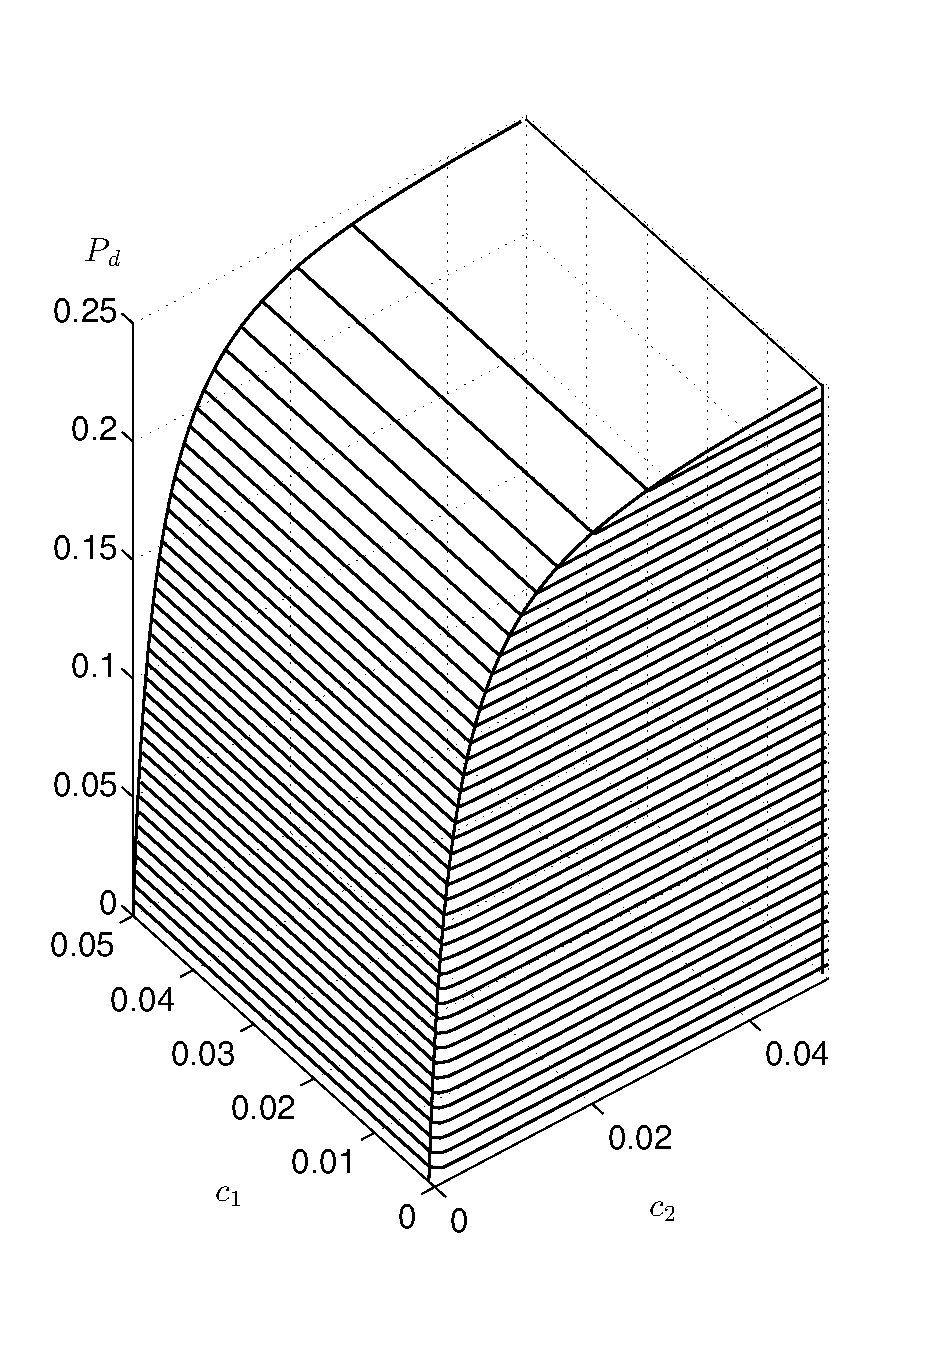
\includegraphics[width=12cm, height=16cm]{4/ROCsurface.eps}
  \caption{M-ROC surface for cyclostationary detector.}
  \label{pic:1221n0}
\end{figure}

